        %%******************************************%%
        %%                                          %%
        %%        Modello di tesi di laurea         %%
        %%            di Andrea Giraldin            %%
        %%                                          %%
        %%             2 novembre 2012              %%
        %%                                          %%
        %%******************************************%%


% I seguenti commenti speciali impostano:
% 1. 
% 2. PDFLaTeX come motore di composizione;
% 3. tesi.tex come documento principale;
% 4. il controllo ortografico italiano per l'editor.

% !TEX encoding = UTF-8
% !TEX TS-program = pdflatex
% !TEX root = tesi.tex
% !TEX spellcheck = it-IT

% PDF/A filecontents
\RequirePackage{filecontents}
\begin{filecontents*}{\jobname.xmpdata}
  \Title{Sviluppo di un modulo software per la gestione degli ordini di acquisto con l'utilizzo di metodi euristici di ottimizzazione ​}
  \Author{Filippo Brugnolaro}
  \Language{it-IT}
  \Subject{ In questo documento viene presentata l'esperienza di stage fatta da Brugnolaro Filippo presso l'azienda Ergon Informatica srl
            alla fine del percorso di laurea triennale ​}
  \Keywords{ottimizzazione\sep euristica\sep algoritmi\sep gestione ordini\sep development ​\sep}
\end{filecontents*}

\documentclass[10pt,                    % corpo del font principale
               a4paper,                 % carta A4
               twoside,                 % impagina per fronte-retro
               openright,               % inizio capitoli a destra
               english,                 
               italian,                 
               ]{book}    

%**************************************************************
% Importazione package
%************************************************************** 

\usepackage{geometry}
\geometry{a4paper, left=30mm, right=30mm, top=31mm, bottom=30mm}

\usepackage[table, dvipsnames]{xcolor}
\definecolor{red}{rgb}{0.6,0,0}
\definecolor{blue}{rgb}{0,0,0.6}
\definecolor{green}{rgb}{0,0.8,0}
\definecolor{cyan}{rgb}{0.0,0.6,0.6}
\definecolor{footer-gray}{HTML}{808080}
\definecolor{light-gray}{gray}{0.6} 
\definecolor{light-grayer}{gray}{0.75} 
\definecolor{lighter-grayer}{gray}{0.85} 
\definecolor{lightest-grayest}{gray}{0.94} 
\definecolor{codegreen}{rgb}{0,0.4,0.2}
\definecolor{codegray}{rgb}{0.5,0.5,0.5}
\definecolor{codepurple}{rgb}{0.58,0,0.82}
\definecolor{backcolour}{rgb}{0.95,0.95,0.96}

\usepackage[normalem]{ulem}

\PassOptionsToPackage{dvipsnames}{xcolor} % colori PDF/A

\usepackage{colorprofiles}

\usepackage[a-2b,mathxmp]{pdfx}[2022/09/15]
                                        % configurazione PDF/A
                                        % validare in https://www.pdf-online.com/osa/validate.aspx

\usepackage{amsmath,amssymb,amsthm}    % matematica

\usepackage[T1]{fontenc}                % codifica dei font:
                                        % NOTA BENE! richiede una distribuzione *completa* di LaTeX

\usepackage[utf8]{inputenc}             % codifica di input; anche [latin1] va bene
                                        % NOTA BENE! va accordata con le preferenze dell'editor

\usepackage[english, italian]{babel}    % per scrivere in italiano e in inglese;
                                        % l'ultima lingua (l'italiano) risulta predefinita

\usepackage{bookmark}                   % segnalibri

\usepackage{caption}                    % didascalie

\usepackage{chngpage,calc}              % centra il frontespizio

\usepackage{csquotes}                   % gestisce automaticamente i caratteri (")

\usepackage{emptypage}                  % pagine vuote senza testatina e piede di pagina

\usepackage{epigraph}			              % per epigrafi

\usepackage{eurosym}                    % simbolo dell'euro

\usepackage{indentfirst}                % rientra il primo paragrafo di ogni sezione

\usepackage{graphicx}                   % immagini

\usepackage{hyperref}                   % collegamenti ipertestuali

\usepackage[binding=5mm]{layaureo}      % margini ottimizzati per l'A4; rilegatura di 5 mm

\usepackage{listings}                   % codici

\usepackage{microtype}                  % microtipografia

\usepackage{mparhack,fixltx2e,relsize}  % finezze tipografiche

\usepackage{nameref}                    % visualizza nome dei riferimenti                                      
\usepackage[font=small]{quoting}        % citazioni

\usepackage{subfig}                     % sottofigure, sottotabelle

\usepackage[italian]{varioref}          % riferimenti completi della pagina

\usepackage{booktabs}                   % tabelle                                       
\usepackage{tabularx}                   % tabelle di larghezza prefissata                                    
\usepackage{longtable}                  % tabelle su più pagine                                        
\usepackage{ltxtable}                   % tabelle su più pagine e adattabili in larghezza
\usepackage{multicol}                   % liste elementi multicolonna

\usepackage[toc, acronym]{glossaries}   % glossario
                                        % per includerlo nel documento bisogna:
                                        % 1. compilare una prima volta tesi.tex;
                                        % 2. eseguire: makeindex -s tesi.ist -t tesi.glg -o tesi.gls tesi.glo
                                        % 3. eseguire: makeindex -s tesi.ist -t tesi.alg -o tesi.acr tesi.acn
                                        % 4. compilare due volte tesi.tex.

\usepackage[backend=biber,style=numeric-comp,hyperref,backref]{biblatex}
                                        % eccellente pacchetto per la bibliografia; 
                                        % produce uno stile di citazione autore-anno; 
                                        % lo stile "numeric-comp" produce riferimenti numerici
                                        % per includerlo nel documento bisogna:
                                        % 1. compilare una prima volta tesi.tex;
                                        % 2. eseguire: biber tesi
                                        % 3. compilare ancora tesi.tex.

\usepackage[Algoritmo]{algorithm}       % algoritmi

\usepackage{algpseudocode}              % pseudocodice


%**************************************************************
% file contenente le impostazioni della tesi
%**************************************************************

%**************************************************************
% Frontespizio
%**************************************************************

% Autore
\newcommand{\myName}{Filippo Brugnolaro}

% Matricola
\newcommand{\myFreshman}{1217321}

\newcommand{\myTitle}{Sviluppo di un modulo software per la gestione degli ordini di acquisto con l'utilizzo di\\metodi euristici di ottimizzazione}

% Tipo di tesi                   
\newcommand{\myDegree}{Tesi di laurea triennale}

% Università             
\newcommand{\myUni}{Università degli Studi di Padova}

% Facoltà       
\newcommand{\myFaculty}{Corso di Laurea in Informatica}

% Dipartimento
\newcommand{\myDepartment}{Dipartimento di Matematica "Tullio Levi-Civita"}

% Titolo del relatore
\newcommand{\profTitle}{Prof. }

% Relatore
\newcommand{\myProf}{Luigi De Giovanni}

% Luogo
\newcommand{\myLocation}{Padova}

% Anno accademico
\newcommand{\myAA}{2021-2022}

% Data discussione
\newcommand{\myTime}{Settembre 2022}

% Azienda
\newcommand{\myCompany}{Ergon Informatica S.R.L.}


%**************************************************************
% Impostazioni di impaginazione
% see: http://wwwcdf.pd.infn.it/AppuntiLinux/a2547.htm
%**************************************************************

\setlength{\parindent}{14pt}   % larghezza rientro della prima riga
\setlength{\parskip}{0pt}   % distanza tra i paragrafi


%**************************************************************
% Impostazioni di biblatex
%**************************************************************

\bibliography{bibliografia} % database di biblatex 

\defbibheading{bibliography} {
    \cleardoublepage
    \phantomsection 
    \addcontentsline{toc}{chapter}{\bibname}
    \chapter*{\bibname\markboth{\bibname}{\bibname}}
}

\setlength\bibitemsep{1.5\itemsep} % spazio tra entry

\DeclareBibliographyCategory{opere}
\DeclareBibliographyCategory{web}

\addtocategory{opere}{womak:lean-thinking}
\addtocategory{web}{site:agile-manifesto}

\defbibheading{opere}{\section*{Riferimenti bibliografici}}
\defbibheading{web}{\section*{Siti Web consultati}}


%**************************************************************
% Impostazioni di caption
%**************************************************************
\captionsetup{
    tableposition=top,
    figureposition=bottom,
    font=small,
    format=hang,
    labelfont=bf
}

%**************************************************************
% Impostazioni di glossaries
%**************************************************************
\makeglossaries

%**************************************************************
% Acronimi
%**************************************************************
%\newacronym[description={\glslink{apig}{Application Program Interface}}]
%    {api}{API}{Application Program Interface}
%
%\newacronym[description={\glslink{umlg}{Unified Modeling Language}}]
%    {uml}{UML}{Unified Modeling Language}

%**************************************************************
% Glossario
%**************************************************************
\newglossaryentry{apig}
{
    name=\glslink{api}{API},
    text=API,
    sort=api,
    description={(\emph{Application Programming Interface})
    Intermediario \textit{software} che permette a due
    applicazioni non correlate di comunicare tra loro}
}

\newglossaryentry{umlg}
{
    name=\glslink{uml}{UML},
    text=UML,
    sort=uml,
    description={(\emph{Unified Model Language})
    \textit{Standard} utilizzato nell'ingegneria del \textit{software}
    per descrivere un sistema informatico, consentendo ai
    vari ruoli (sviluppatore, tester, analista,ecc.) di
    comunicare tramite lo stesso linguaggio. Si avvale di
    diversi tipi di diagrammi, statici e dinamici,
    per fornire diverse viste di uno stesso sistema \cite{site:def-uml}}
}

\newglossaryentry{erpg}
{
    name=\glslink{erp}{ERP},
    text=ERP,
    sort=erp,
    description={(\emph{Enterprise Resource Planning})
    Tipologia di \textit{software} che integra tutti i processi
    di business rilevanti di un'azienda e tutte le funzioni
    aziendali, ad esempio vendite, acquisti, gestione magazzino,
    finanza, contabilità etc. \cite{site:wiki}}
}

\newglossaryentry{.netg}
{
    name=\glslink{.netframework}{.NET Framework},
    text=.NET Framework,
    sort=.netframework,
    description={Ambiente di esecuzione runtime
    della piattaforma tecnologica \textit{.NET} in cui
    vengono gestite le applicazioni destinate allo stesso
    \textit{.NET Framework} \cite{site:wiki}}
}

\newglossaryentry{devexpressg}
{
    name=\glslink{devexpress}{DevExpress},
    text=DevExpress,
    sort=devexpress,
    description={\textit{Framework} utile per lo sviluppo
    di applicazioni desktop \cite{site:devexpress-docs}}
}

\newglossaryentry{serverconsolidationg}
{
    name=\glslink{serverconsolidation}{Server Consolidation},
    text=server consolidation,
    sort=serverconsolidation,
    description={Approccio all'utilizzo efficiente
    delle risorse dei \textit{server} dei computer al fine di
    ridurre il numero totale di \textit{server} o posizioni di
    \textit{server} richiesti da un'organizzazione \cite{site:def-server-cons}}
}

\newglossaryentry{ergdisg}
{
    name=\glslink{ergdis}{ERGDIS},
    text=ERGDIS,
    sort=ergdis,
    description={\textit{Software} proprietario dell'azienda \textit{\myCompany}}
}

\newglossaryentry{stakeholdersg}
{
    name=\glslink{stakeholder}{Stakeholders},
    text=stakeholders,
    sort=stakeholders,
    description={Coloro che a vario titolo hanno influenza su un
    prodotto o su un progetto}
}

\newglossaryentry{windowsformg}
{
    name=\glslink{windowsform}{Windows form},
    text=Windows form,
    sort=windowsform,
    description={Applicazione basata su eventi
    supportata da \textit{.NET Framework} di \textit{Microsoft} \cite{site:wiki}}
}

\newglossaryentry{ricercaoperativag}
{
    name=\glslink{ricercaoperativa}{Ricerca Operativa},
    text=Ricerca Operativa,
    sort=ricercaoperativa,
    description={Scienza che fornisce strumenti matematici e algoritmici di
    supporto alle attività decisionali in cui occorre gestire
    e coordinare attività e risorse limitate \cite{site:wiki}}
}

\newglossaryentry{ammissibileg}
{
    name=\glslink{ammissibile}{Soluzione Ammissibile},
    text=ammissibile,
    sort=ammissibile,
    description={Soluzione che rispetta tutti i vincoli del problema}
}

\newglossaryentry{astrazioneg}
{
    name=\glslink{astrazione}{Astrazione},
    text=astrazione,
    sort=astrazione,
    description={Applicazione del metodo logico di astrazione nella strutturazione della
    descrizione dei sistemi informatici complessi, per facilitarne la progettazione e
    manutenzione o la stessa comprensione. La pratica consiste nel presentare il
    sistema, ad esempio un pezzo di codice sorgente o uno scambio di trasmissioni di
    dati, in maniera ridotta ai soli dettagli considerati essenziali all’interesse specifico,
    ad esempio raggruppando il codice in una funzione o formalizzando un protocollo
    di comunicazione \cite{site:wiki}}
}

\newglossaryentry{businessintelligenceg}
{
    name=\glslink{businessintelligence}{Business Intelligence},
    text=Business Intelligence,
    sort=businessintelligence,
    description={Con la locuzione \textit{business intelligence}
    (\textit{BI}), ci si può solitamente riferire a: un insieme di processi aziendali per raccogliere dati ed analizzare
    informazioni strategiche, la tecnologia utilizzata per realizzare questi processi
    oppure le informazioni ottenute come risultato di questi processi \cite{site:wiki}}
}

\newglossaryentry{debugg}
{
    name=\glslink{debug}{Debug},
    text=debug,
    sort=debug,
    description={Termine che indica l’attività che
    consiste nell’individuazione e correzione da parte del programmatore di uno o più
    errori (\textit{bug}) rilevati nel \textit{software}, direttamente in fase di programmazione oppure
    a seguito della fase di \textit{testing} o dell’utilizzo finale del programma stesso \cite{site:wiki}}
}

\newglossaryentry{debuggerg}
{
    name=\glslink{debugger}{Debugger},
    text=debugger,
    sort=debugger,
    description={Programma/\textit{software} specificatamente
    progettato per l’analisi e l’eliminazione dei \textit{bug} (\textit{debugging}), ovvero errori di
    programmazione interni al codice di altri programmi \cite{site:wiki}}
}

\newglossaryentry{ereditarietag}
{
    name=\glslink{ereditarietà}{Ereditarietà},
    text=ereditarietà,
    sort=ereditarietà,
    description={Uno dei principi fondamentali della programmazione ad oggetti. In
    generale, essa rappresenta un meccanismo che consente di creare nuovi oggetti
    che siano basati su altri già definiti. Si definisce oggetto figlio 
    quello che eredita tutte o parte delle proprietà e dei metodi definiti nell’oggetto
    padre \cite{site:wiki}}
}

\newglossaryentry{ideg}
{
    name=\glslink{ide}{IDE},
    text=IDE,
    sort=ide,
    description={(\textit{Integrated Development Environment})
    \textit{Software} che aiuta gli sviluppatori nella fase di programmazione con vari strumenti
    di analisi del codice e integrazione di altre componenti \cite{site:wiki}}
}

\newglossaryentry{intellisenseg}
{
    name=\glslink{intellisense}{IntelliSense},
    text=intellisense,
    sort=intellisense,
    description={Forma di completamento automatico resa popolare da Visual Studio.
    Serve inoltre come documentazione per i
    nomi delle variabili, delle funzioni e dei metodi usando metadati. L’uso
    dell’IntelliSense è un metodo conveniente per visualizzare la descrizione delle
    funzioni, in particolar modo la lista dei loro parametri. Questa tecnologia riesce
    a velocizzare lo sviluppo del \textit{software} riducendo la quantità di \textit{input} attraverso
    la tastiera \cite{site:wiki}}
}

\newglossaryentry{logg}
{
    name=\glslink{log}{Log},
    text=log,
    sort=log,
    description={\textit{File} su cui sono registrati eventi caratteristici dell’applicazione e che fungono
    in certi casi da vero e proprio protocollo di entrata e di uscita. Ad esempio, in
    programmazione, il \textit{file} di \textit{log} evidenzia il tipo di errore e il punto nel codice
    da parte dell’\textit{IDE} \cite{site:wiki}}
}

\newglossaryentry{oltpg}
{
    name=\glslink{oltp}{OLTP},
    text=OLTP,
    sort=oltp,
    description={(\textit{Online transaction processing}) è un insieme di tecniche \textit{software} utilizzate per
    la gestione di applicazioni orientate alle transazioni \cite{site:wiki}}
}

\newglossaryentry{polimorfismog}
{
    name=\glslink{polimorfismo}{Polimorfismo},
    text=polimorfismo,
    sort=polimorfismo,
    description={Termine usato in senso generico
    per riferirsi a espressioni che possono rappresentare valori di diversi tipi (dette
    espressioni polimorfiche). In un linguaggio non tipizzato, tutte le espressioni
    sono intrinsecamente polimorfiche. Nel contesto della programmazione orientata
    agli oggetti, si riferisce al fatto che una espressione il cui tipo sia descritto da
    una classe A può assumere valori di un qualunque tipo descritto da una classe B
    sottoclasse di A (polimorfismo per inclusione) \cite{site:wiki}}
}

\newglossaryentry{refactoringg}
{
    name=\glslink{refactoring}{Refactoring},
    text=refactoring,
    sort=refactoring,
    description={Tecnica per modificare la struttura interna di porzioni di codice
    senza modificarne il comportamento esterno, applicata per migliorare alcune
    caratteristiche non funzionali del \textit{software} \cite{Addison-Wesley:software-engineering}}
}

\newglossaryentry{ricercalocaleg}
{
    name=\glslink{ricercalocale}{Ricerca locale},
    text=ricerca locale,
    sort=ricercalocale,
    description={Algoritmo che si basa sull’idea di migliorare
    una soluzione iniziale esplorandone un intorno
    opportunamente definito. Se l’ottimizzazione
    dell’intorno produce una soluzione migliorante
    il procedimento viene ripetuto
    considerando come soluzione corrente la soluzione
    appena determinata. L’algoritmo termina se non è più
    possibile trovare soluzioni miglioranti, quindi al
    raggiungimento di un ottimo locale, oppure al
    raggiungimento di un numero
    determinato di iterazioni o di un tempo massimo di esecuzione \cite{site:dispense-de-giovanni}}
}

\newglossaryentry{javag}
{
    name=\glslink{java}{Java},
    text=Java,
    sort=java,
    description={linguaggio di programmazione
    \textit{general-purpose} ad livello, basato su classi, orientato alla programmazione ad oggetti e
    progettato
    per avere il minor numero di dipendenze di implementazione
    possibile \cite{site:wiki}}
}

\newglossaryentry{linqg}
{
    name=\glslink{linq}{LINQ},
    text=LINQ,
    sort=linq,
    description={(\textit{Language-Integrated Query})
    Insieme di tecnologie basate sull'integrazione delle funzionalità di query direttamente nel linguaggio C\# \cite{site:wiki}}
}

\newglossaryentry{visualbasicg}
{
    name=\glslink{visualbasic}{Visual Basic},
    text=Visual Basic,
    sort=visualbasic,
    description={Linguaggio di programmazione \textit{event driven} creato da \textit{Microsoft} \cite{site:wiki}}
}

\newglossaryentry{C++g}
{
    name=\glslink{c++}{C++},
    text=C++,
    sort=c++,
    description={Linguaggio di programmazione
    general purpose sviluppato come evoluzione del linguaggio C inserendo la programmazione orientata agli oggetti}
}

\newglossaryentry{JUnitg}
{
    name=\glslink{junit}{JUnit},
    text=JUnit,
    sort=junit,
    description={\textit{Framework} di \textit{unit testing} per il linguaggio di programmazione \textit{Java}}
}

\newglossaryentry{aaag}
{
    name=\glslink{aaa}{Arrange-Act-Assert},
    text=AAA,
    sort=aaa,
    description={\textit{Pattern} per scrivere \textit{test} di unità che abbiano una struttura uniforme. Questo li rende anche facilmente leggibili e comprensibili}
}

\newglossaryentry{nosqlg}
{
    name=\glslink{nosql}{NoSQL},
    text=NoSQL,
    sort=nosql,
    description={Tipo di \textit{database} realizzati per modelli di dati specifici con schemi flessibili. Sono molto utilizzati per la facilità di sviluppo, le funzionalità che offrono e la scalabilità delle prestazioni \cite{site:wiki}}
}

\newglossaryentry{databaseg}
{
    name=\glslink{database}{Database},
    text=database,
    sort=database,
    description={Archivio di dati strutturato in modo da razionalizzare la gestione e l'aggiornamento delle informazioni e da permettere lo svolgimento di ricerche complesse \cite{site:def-db}}
}

\newglossaryentry{preprocessingg}
{
    name=\glslink{preprocessing}{Pre-processing},
    text=pre-processing,
    sort=preprocessing,
    description={Consiste nella manipolazione o nell'eliminazione
    dei dati prima che vengano utilizzati al fine di
    garantire o migliorare le prestazioni \cite{site:wiki}}
}

\newglossaryentry{sqlg}
{
    name=\glslink{sql}{SQL},
    text=SQL,
    sort=sql,
    description={(Structured Query Language) Linguaggio standardizzato per \textit{database} basati sul modello relazionale}
}

\newglossaryentry{milestoneg}
{
    name=\glslink{milestone}{Milestone},
    text=milestone,
    sort=milestone,
    description={Consiste in importanti traguardi intermedi nello svolgimento di un progetto}
}

\newglossaryentry{entityframeworkg}
{
    name=\glslink{entityframework}{Entity Framework},
    text=Entity Framework,
    sort=entityframework,
    description={Mappatore di \textit{database} di oggetti per l'ambiente \textit{.NET} \cite{site:docs-ef}}
}

\newglossaryentry{rdbmsg}
{
    name=\glslink{rdbms}{Relational Database Management System},
    text=RDBMS,
    sort=rdbms,
    description={Sistema \textit{software} progettato per consentire la creazione, la manipolazione e l'interrogazione efficiente di \textit{database}, per questo detto anche "gestore o motore del \textit{database}". È basato sul modello relazionale \cite{site:wiki}}
} % database di termini


%**************************************************************
% Impostazioni di graphicx
%**************************************************************
\graphicspath{{immagini/}} % cartella dove sono riposte le immagini


%**************************************************************
% Impostazioni di hyperref
%**************************************************************
\hypersetup{
    %hyperfootnotes=false,
    %pdfpagelabels,
    draft,	% = elimina tutti i link (utile per stampe in bianco e nero)
    colorlinks=true,
    linktocpage=true,
    pdfstartpage=1,
    pdfstartview=,
    % decommenta la riga seguente per avere link in nero (per esempio per la stampa in bianco e nero)
    colorlinks=false, linktocpage=false, pdfborder={0 0 0}, pdfstartpage=1, pdfstartview=FitV,
    breaklinks=true,
    pdfpagemode=UseNone,
    pageanchor=true,
    pdfpagemode=UseOutlines,
    plainpages=false,
    bookmarksnumbered,
    bookmarksopen=true,
    bookmarksopenlevel=1,
    hypertexnames=true,
    pdfhighlight=/O,
    %nesting=true,
    %frenchlinks,
    urlcolor=webbrown,
    linkcolor=RoyalBlue,
    citecolor=webgreen,
    %pagecolor=RoyalBlue,
    %urlcolor=Black, linkcolor=Black, citecolor=Black, %pagecolor=Black,
    pdftitle={\myTitle},
    pdfauthor={\textcopyright\ \myName, \myUni, \myFaculty},
    pdfsubject={},
    pdfkeywords={},
    pdfcreator={pdfLaTeX},
    pdfproducer={LaTeX}
}

%**************************************************************
% Impostazioni di itemize
%**************************************************************
\renewcommand{\labelitemi}{$\ast$}

%\renewcommand{\labelitemi}{$\bullet$}
%\renewcommand{\labelitemii}{$\cdot$}
%\renewcommand{\labelitemiii}{$\diamond$}
%\renewcommand{\labelitemiv}{$\ast$}


%**************************************************************
% Impostazioni di listings
%**************************************************************
\lstset{
    language=[LaTeX]Tex,%C++,
    keywordstyle=\color{RoyalBlue}, %\bfseries,
    basicstyle=\small\ttfamily,
    %identifierstyle=\color{NavyBlue},
    commentstyle=\color{Green}\ttfamily,
    stringstyle=\rmfamily,
    numbers=none, %left,%
    numberstyle=\scriptsize, %\tiny
    stepnumber=5,
    numbersep=8pt,
    showstringspaces=false,
    breaklines=true,
    frameround=ftff,
    frame=single
} 


%**************************************************************
% Impostazioni di xcolor
%**************************************************************
\definecolor{webgreen}{rgb}{0,.5,0}
\definecolor{webbrown}{rgb}{.6,0,0}


%**************************************************************
% Altro
%**************************************************************

\newcommand{\omissis}{[\dots\negthinspace]} % produce [...]

% eccezioni all'algoritmo di sillabazione
\hyphenation
{
    ma-cro-istru-zio-ne
    gi-ral-din
}

\newcommand{\sectionname}{sezione}
\addto\captionsitalian{\renewcommand{\figurename}{Figura}
                       \renewcommand{\tablename}{Tabella}}

\newcommand{\glsfirstoccur}{\ap{{[g]}}}

\newcommand{\intro}[1]{\emph{\textsf{#1}}}

%**************************************************************
% Environment per ``rischi''
%**************************************************************
\newcounter{riskcounter}                % define a counter
\setcounter{riskcounter}{0}             % set the counter to some initial value

%%%% Parameters
% #1: Title
\newenvironment{risk}[1]{
    \refstepcounter{riskcounter}        % increment counter
    \par \noindent                      % start new paragraph
    \textbf{\arabic{riskcounter}. #1}   % display the title before the 
                                        % content of the environment is displayed 
}{
    itempar\medskip
}

\newcommand{\riskname}{Rischio}

\newcommand{\riskdescription}[1]{\textbf{\\Descrizione:} #1.}

\newcommand{\risksolution}[1]{\textbf{\\Soluzione:} #1.}

%**************************************************************
% Environment per ``use case''
%**************************************************************
\newcounter{usecasecounter}             % define a counter
\setcounter{usecasecounter}{0}          % set the counter to some initial value

%%%% Parameters
% #1: ID
% #2: Nome
\newenvironment{usecase}[2]{
    \renewcommand{\theusecasecounter}{\usecasename #1}  % this is where the display of 
                                                        % the counter is overwritten/modified
    \refstepcounter{usecasecounter}             % increment counter
    \vspace{10pt}
    \par \noindent                              % start new paragraph
    {\large \textbf{\usecasename #1: #2}}       % display the title before the 
                                                % content of the environment is displayed 
    \medskip
}{
    \medskip
}

\newcommand{\usecasename}{UC}

\newcommand{\usecaseactors}[1]{\textbf{\\Attori principali:} #1. \vspace{4pt}}
\newcommand{\usecasepre}[1]{\textbf{\\Pre-condizione:} #1. \vspace{4pt}}
\newcommand{\usecasedesc}[1]{\textbf{\\Descrizione:} #1. \vspace{4pt}}
\newcommand{\usecasepost}[1]{\textbf{\\Post-condizione:} #1. \vspace{4pt}}
\newcommand{\usecaseprinc}[1]{\textbf{\\Scenario principale:} #1 \vspace{4pt}}
\newcommand{\usecasealt}[1]{\vspace{-16pt} \textbf{\\Scenario alternativo:} #1 \vspace{4pt}}

%**************************************************************
% Environment per ``namespace description''
%**************************************************************

\newenvironment{namespacedesc}{
    \vspace{10pt}
    \par \noindent                              % start new paragraph
    \begin{description} 
}{
    \end{description}
    \medskip
}

% Custom by Filippo

\newcommand{\classdesc}[2]{\item[\textbf{#1:}] #2}

\newcommand{\req}[3]{\centering #1 & #2 & \centering #3 \arraybackslash\\ \hline}

\newcommand{\reqval}[4]{\centering #1 & #2 & \centering #3 & \centering #4 \arraybackslash\\ \hline}

\newcommand{\reqsum}[4]{\centering #1 & \centering #2 & \centering #3 & \centering #4 \arraybackslash\\ \hline}

\renewcommand{\listalgorithmname}{Lista degli algoritmi}

\renewcommand{\algorithmicforall}{\textbf{for each}}

\usepackage{fancyhdr}                   % per modificare dimensioni,margini, intestazioni e righe a piè di pagina

% mettere sottosezioni negli header
%\renewcommand{\subsectionmark}[1]{\markright{\MakeUppercase{\thesubsection.\ #1}}}

\fancypagestyle{plain}{
    
    \fancyhf{}                          % cancella tutti i campi di intestazione e piè di pagina

    \fancyhead{}
%    \fancyhead[LO, RE]{\leftmark}
    \fancyfoot[C]{\thepage}
    \fancypagestyle{plain}{\fancyhead{}}

    \fancyfoot[C]{\thepage{}}           % numero della pagina nel footer

    \renewcommand{\headrulewidth}{0pt}  % linea orizzontale in posizione top della pagina (se è 0, non c'è la linea)
    \renewcommand{\footrulewidth}{0pt}  % linea orizzontale in posizione bottom della pagina (se è 0, non c'è la linea)
}
\pagestyle{plain}

\newcommand{\fval}[4]{\centering#1 & \centering #2/1300 & \centering #3 & \centering #4 \arraybackslash\\ \hline}

\usepackage{multirow}

\newcommand{\valtest}[3]{\centering #1 & & \centering #2 & \centering #3 \arraybackslash\\ \cline{1-1} \cline{3-4}}                     % file con le impostazioni personali

\begin{document}
%**************************************************************
% Materiale iniziale
%**************************************************************
\frontmatter
% !TEX encoding = UTF-8
% !TEX TS-program = pdflatex
% !TEX root = ../tesi.tex

%**************************************************************
% Frontespizio 
%**************************************************************
\begin{titlepage}

\begin{center}

\begin{LARGE}
\textbf{\myUni}\\
\end{LARGE}

\vspace{10pt}

\begin{Large}
\textsc{\myDepartment}\\
\end{Large}

\vspace{10pt}

\begin{large}
\textsc{\myFaculty}\\
\end{large}

\vspace{30pt}
\begin{figure}[htbp]
\begin{center}

\includegraphics[height=6cm]{logo-unipd}
\end{center}
\end{figure}
\vspace{30pt} 

\begin{LARGE}
\begin{center}
\textbf{\myTitle}\\
\end{center}
\end{LARGE}

\vspace{10pt} 

\begin{large}
\textsl{\myDegree}\\
\end{large}

\vspace{40pt} 

\begin{large}
\begin{flushleft}
\textit{Relatore}\\ 
\vspace{5pt} 
\profTitle \myProf
\end{flushleft}

\vspace{0pt} 

\begin{flushright}
\textit{Laureando}\\ 
\vspace{5pt} 
\myName
\end{flushright}
\end{large}

\vspace{40pt}

\line(1, 0){338} \\
\begin{normalsize}
\textsc{Anno Accademico \myAA}
\end{normalsize}

\end{center}
\end{titlepage} 
% !TEX encoding = UTF-8
% !TEX TS-program = pdflatex
% !TEX root = ../tesi.tex

%**************************************************************
% Colophon
%**************************************************************
\clearpage
\phantomsection
\thispagestyle{empty}

\hfill

\vfill

\noindent\myName: \textit{Sviluppo di un modulo software per la gestione degli ordini di acquisto con l'utilizzo di metodi euristici di ottimizzazione,}
\myDegree,
\textcopyright\ \myTime.
%% !TEX encoding = UTF-8
% !TEX TS-program = pdflatex
% !TEX root = ../tesi.tex

%**************************************************************
% Dedica
%**************************************************************
\cleardoublepage
\phantomsection
\thispagestyle{empty}
\pdfbookmark{Dedica}{Dedica}

\vspace*{3cm}

\begin{center}
Lorem ipsum dolor sit amet, consectetuer adipiscing elit. \\ \medskip
--- Oscar Wilde    
\end{center}

\medskip

\begin{center}
Dedicato a ...
\end{center}

% !TEX encoding = UTF-8
% !TEX TS-program = pdflatex
% !TEX root = ../tesi.tex

%**************************************************************
% Sommario
%**************************************************************
\cleardoublepage
\phantomsection
\pdfbookmark{Sommario}{Sommario}
\begingroup
\let\clearpage\relax
\let\cleardoublepage\relax
\let\cleardoublepage\relax

\chapter*{Sommario}

Il presente documento descrive il lavoro svolto durante il periodo di stage, della durata di circa trecento ore, dal laureando Pinco Pallino presso l'azienda Azienda S.p.A.
Gli obbiettivi da raggiungere erano molteplici.\\
In primo luogo era richiesto lo sviluppo di ...
In secondo luogo era richiesta l'implementazione di un ... 
Tale framework permette di registrare gli eventi di un controllore programmabile, quali segnali applicati 
Terzo ed ultimo obbiettivo era l'integrazione ...

%\vfill
%
%\selectlanguage{english}
%\pdfbookmark{Abstract}{Abstract}
%\chapter*{Abstract}
%
%\selectlanguage{italian}

\endgroup			

\vfill


% !TEX encoding = UTF-8
% !TEX TS-program = pdflatex
% !TEX root = ../tesi.tex

%**************************************************************
% Ringraziamenti
%**************************************************************
\cleardoublepage
\phantomsection
\pdfbookmark{Ringraziamenti}{ringraziamenti}

\begin{flushright}
	{
	\slshape
	La disumanità del computer sta nel fatto che,\\
	una volta programmato e messo in funzione,\\
	si comporta in maniera perfettamente onesta. \\
	\medskip
	--- Isaac Asimov
	}
	\end{flushright}
	
	\bigskip
	
	\begingroup
	\let\clearpage\relax
	\let\cleardoublepage\relax
	\let\cleardoublepage\relax
	
	\chapter*{Ringraziamenti}
	
	\noindent
	\textit{In primis vorrei esprimere la mia gratitudine al
			Professor Luigi De Giovanni, relatore della mia tesi,
			per la disponibilità e l'aiuto fornitomi durante la
			stesura.}\\
	
	\noindent
	\textit{Desidero ringraziare con affetto la mia famiglia
			per tutto il sostegno e la vicinanza dimostrata
			in ogni momento e per non avermi mai fatto mancare
			nulla durante gli anni di studio.}\\
	
	\noindent
	\textit{Vorrei ringraziare i miei amici che mi sono
			stati vicini e mi hanno accompagnato in questi anni,
			soprattutto nei momenti difficili.}\\
	
	\noindent
	\textit{Infine desidero ringraziare in maniera speciale il mio amico
			Alessandro, che mi ha reso lo studio meno faticoso e con cui
			ho passato dei bei momenti, e Linpeng, che mi ha pazientemente
			guidato all'inizio del corso di laurea.}\\
	\bigskip
	
	\noindent\textit{\myLocation, \myTime}
	\begin{flushright}
	\myName
	\end{flushright}
	
	\endgroup


% !TEX encoding = UTF-8
% !TEX TS-program = pdflatex
% !TEX root = ../tesi.tex

%**************************************************************
% Indici
%**************************************************************
\cleardoublepage
\pdfbookmark{\contentsname}{tableofcontents}
\setcounter{tocdepth}{2}
\tableofcontents
%\markboth{\contentsname}{\contentsname} 
\clearpage

\begingroup 
    \let\clearpage\relax
    \let\cleardoublepage\relax
    \let\cleardoublepage\relax
    %*******************************************************
    % Elenco delle figure
    %*******************************************************    
    \phantomsection
    \pdfbookmark{\listfigurename}{lof}
    \listoffigures

    %*******************************************************
    % Elenco delle tabelle
    %*******************************************************
    \phantomsection
    \pdfbookmark{\listtablename}{lot}
    \listoftables

    %*******************************************************
    % Elenco degli algorimi
    %*******************************************************
    \renewcommand{\listalgorithmname}{Elenco degli algoritmi}
    \phantomsection
    \pdfbookmark{\listtablename}{lot}
    \listofalgorithms
        
    
        
    \vspace*{8ex}
\endgroup

\cleardoublepage

\cleardoublepage

%**************************************************************
% Materiale principale
%**************************************************************
\mainmatter
% !TEX encoding = UTF-8
% !TEX TS-program = pdflatex
% !TEX root = ../tesi.tex

%**************************************************************
\newgeometry{a4paper, left=30mm, right=30mm, top=5mm, bottom=30mm}

\chapter{Introduzione}
\label{cap:introduzione}
%**************************************************************

\noindent \intro{In questo capitolo si introduce brevemente l'azienda ospitante e il progetto affrontato.}\\

%Introduzione al contesto applicativo.\\

%\noindent Esempio di utilizzo di un termine nel glossario \\
%\gls{api}. \\

%\noindent Esempio di citazione in linea \\
%\cite{site:agile-manifesto}. \\

%\noindent Esempio di citazione nel pie' di pagina \\
%citazione\footcite{womak:lean-thinking} \\

%**************************************************************
\section{L'azienda}

\noindent{\myCompany} \cite{siteB:ergon-informatica}
(da qui in poi
\textit{"Ergon Informatica"}) è un'azienda italiana, fondata nel 1988, 
con sede a Castelfranco Veneto.\\
Essa si occupa principalmente di soluzioni gestionali per piccole e medie imprese e dello sviluppo di
\textit{software \gls{erpg}} $^{[g]}$ (\textit{Enterprise Resource Planning}) per i settori dell'alimentare e dei trasporti,
ma completa l'offerta con la vendita di prodotti
\textit{hardware}, servizi \textit{web} e \textit{hosting}, nonché con progetti di \textit{\gls{serverconsolidationg}} $^{[g]}$ e virtualizzazione di
sistemi.
L'azienda inoltre si è sviluppata in maniera costante negli anni e oggi può vantare una posizione di tutto rispetto tra le aziende dello stesso settore.
Attualmente fanno parte della stessa gestione:

\begin{itemize}
    \item \textit{Ergon Informatica S.R.L.}: che si occupa del \textit{software};
    \item \textit{Ergon S.R.L.}: che si occupa dei servizi tecnologici;
    \item \textit{Ergon Servizi S.R.L.}: che si occupa dei servizi amministrativi, logistici e di \textit{marketing} delle altre due parti.
\end{itemize}
Il logo dell'azienda è illustrato in Figura \ref{fig:logo}.
\vfill
\begin{figure}[!h]
    \centering
    
\includegraphics[width=0.8\columnwidth]{loghi/Ergon_Logo.pdf}
    \caption{Logo \myCompany}
    \label{fig:logo}
\end{figure}
\vfill
\noindent Il prodotto di proprietà dell'azienda è \textit{\gls{ergdisg}} $^{[g]}$, sistema \textit{\gls{erpg}}
il cui insieme dei moduli copre ogni aspetto della conduzione aziendale.
Alcuni di essi, inoltre, si possono interfacciare con dispositivi automatici presenti in azienda, come, ad esempio,
linee di confezionamento o \textit{robot}.

\newgeometry{a4paper, left=30mm, right=30mm, top=31mm, bottom=30mm}
\newpage
\noindent In particolare  vengono gestiti compiti che si dislocano in vari ambiti e
i moduli vengono dunque raggruppati nelle seguenti categorie:
\begin{multicols}{2}
\begin{itemize}
    \item Amministrazione e Finanza
    \item Controllo di Gestione
    \item Area Acquisti
    \item Logistica
    \item Vendite
    \item Produzione
\end{itemize}
\begin{itemize}
    \item \textit{Web}
    \item \textit{\gls{businessintelligenceg}} $^{[g]}$
    \item Qualità
    \item Gestione Archivi e Documentazione
    \item Pianificazione Consegne
    \item Area \textit{Mobile}
\end{itemize}
\end{multicols}

\noindent In generale, l'azienda può contare su una vasta gamma di clienti,
in quanto i prodotti vengono sviluppati in base alle esigenze di ognuno di essi.
Il prodotto viene prima creato a partire da uno \textit{standard}
a cui vengono successivamente aggiunte le varie funzionalità.\\
Il fatto di poter creare dei prodotti \textit{custom}, rende l'azienda altamente competitiva
e, proprio per questo motivo, il contatto
continuo con gli \textit{\gls{stakeholdersg}} $^{[g]}$ è molto importante, sia per accontentare le loro richieste che per
far evolvere \textit{\gls{ergdisg}} in una maniera tale da essere sempre in linea con le esigenze di mercato.


%**************************************************************
\section{L'idea dello stage}
\noindent Lo \textit{stage} proposto consiste nella progettazione e nello sviluppo di un modulo \textit{software} volto
ad assistere l'azienda nella fase di approvvigionamento dei prodotti dai propri fornitori, supportandola nello scegliere
da quale fornitore e quando acquistare i prodotti.
\noindent Questa nuova funzionalità andrebbe ad ottimizzare un modulo già esistente facente parte della
gestione dell'\textit{Area Acquisti}.\\
In pratica il modulo attuale, per ogni prodotto da ordinare, prende in considerazione l'ultima data d'ordine disponibile prima dell'inizio
dell'effettiva copertura del fabbisogno del prodotto stesso. Questo dunque non garantirebbe con certezza una scelta ottimale
in relazione alle possibilità d'ordine fornite dagli appositi listini e calendario dei fornitori.\\

\noindent Data la natura combinatoria del problema, che richiede di scegliere il mix migliore di acquisti da vari listini, il nuovo modulo dovrà fornire in tempi ragionevoli una "buona soluzione"
del problema, ovvero tendente il più possibile all'ottimo, e dovrà integrarsi con l'intero sistema \textit{\gls{ergdisg}}.\\

\noindent È previsto inoltre che i dati, su cui si è eseguita l'ottimizzazione e il confronto dei risultati, vengano visualizzati tramite un'apposita
interfaccia grafica che verrà sviluppata in linea con l'ambiente di sviluppo dell'azienda (\textit{\gls{.netg}} $^{[g]}$ e \textit{\gls{devexpressg}} $^{[g]}$).


%**************************************************************
\section{Descrizione dello \textit{stage}}

%**************************************************************
\subsection{Introduzione}
\label{sec:descrizione-stage-intro}

\noindent Lo \textit{stage} consiste nello sviluppo di un algoritmo di ottimizzazione che riesca a diminuire la spesa dell'azienda per gli approvviogionamenti.\\
L'algoritmo dovrà ottimizzare i risultati calcolati da un modulo preesistente, facente parte della gestione dell'\textit{Area Acquisti}, il quale
consiglia di procedere con gli acquisti con una priorità basata sull'ultima data d'ordine disponibile.\\
\noindent La scelta dell'attuale modulo infatti porterebbe a non considerare:
\begin{itemize}
    \item \textbf{l'andamento del mercato}: i prezzi sono variabili e dipendono dal periodo nel quale si comprano i prodotti;
    \item \textbf{i bonus}: i fornitori possono garantire dei bonus in base al raggiungimento di determinati obiettivi di rapporti commerciali.
\end{itemize}
\noindent Facciamo un esempio per chiarire in maniera esplicita perchè si devono andare a considerare parametri come questi. Il problema
è molto semplificato e verrà discusso nei capitoli successivi.\\

%comando arraystretch
\renewcommand{\arraystretch}{1.2}

\begin{table}[!h]
    \begin{center}
        \begin{tabular}{c c c c}
            Articolo & Quantità & Data inizio copertura & Data fine copertura\\
            FEG10 & 2 & 01/07/2022 & 07/07/2022\\
            FRE02 & 3 & 06/07/2022 & 07/07/2022\\
        \end{tabular}
        \vspace{0.3cm}
        \caption{Esempio - Fabbisogni}
    \end{center}
\end{table}
\begin{table}[!h]
        \begin{center}
            \begin{tabular}{c c c c c}
                Articolo & Fornitore & Data inizio validità & Data fine validità & Prezzo(€)\\
                FEG10 & 47040 & 15/06/2022 & 21/06/2022 & 9.50\\
                FRE02 & 47040 & 15/06/2022 & 21/06/2022 & 10.00\\
                FEG10 & 46613 & 22/06/2022 & 31/12/9999 & 10.00\\
                FRE02 & 46613 & 22/06/2022 & 31/12/9999 & 9.50
            \end{tabular}
            \vspace{0.3cm}
            \caption{Esempio - Listino Prezzi}
        \end{center}
\end{table}
\begin{table}[!h]
    \begin{center}
        \begin{tabular}{c c c c}
            Articolo & Fornitore & Data spedizione & Data di arrivo\\
            FEG10 & 47040 & 17/06/2022 & 17/06/2022\\
            FRE02 & 47040 & 19/06/2022 & 19/06/2022\\
            FEG10 & 46613 & 31/06/2022 & 31/06/2022\\
            FRE02 & 46613 & 03/07/2022 & 03/07/2022\\
        \end{tabular}
        \vspace{0.3cm}
        \caption{Esempio - Calendario spedizioni}
    \end{center}
\end{table}

\noindent Il modulo attuale avrebbe sicuramente ordinato entrambi gli articoli dal fornitore \textit{46613},
per un totale di 48.50€. Tuttavia è evidente che non è la miglior soluzione.
Infatti sarrebbe stato opportuno ordinare l'articolo \textit{FEG10} dal fornitore \textit{47040} e il
\textit{FRE02} dal fornitore \textit{46613}, ottenendo dunque un totale di 47.50€.\\
Sebbene possa sembrare un risparmio minimo e trascurabile, se applicato a enormi quantità, può
diventare un notevole risparmio di risorse.\\

\noindent Dopo queste considerazioni, è chiaro come il modulo preesistente non garantisca necessariamente la miglior soluzione in termini economici ed è il motivo per il quale
si è deciso di realizzare un nuovo modulo.\\

\noindent Inoltre, i risultati devono poter essere visualizzati tramite una \textit{\gls{windowsformg}} $^{[g]}$ in cui si dovrà far scegliere all'utente
anche le date entro cui si vuole fare l'analisi.\\

\noindent Per l'azienda, lo \textit{stage}, di cui si riporta in questa tesi, rappresenta un'opportunità per fornire un servizio aggiuntivo ai propri clienti, ma serve anche per avere una base
dalla quale poter eventualmente estendere il modulo con nuovi algoritmi più efficienti.
%**************************************************************
\newpage
\subsection{Obiettivi}
\label{sec:obiettivi}
\noindent Nella Tabella \ref{tab:obiettivi} vengono elencati tutti gli obiettivi previsti dallo \textit{stage}, dove
i codici obiettivo con prefisso \textit{OB} rappresentano gli obiettivi obbligatori, \textit{DE} quelli desiderabili
e \textit{FA} quelli facoltativi.

\renewcommand{\arraystretch}{1.55}

% tabella con i risultati
\begin{center}
    \begin{longtable}{m{3cm}m{9cm}}
    \caption{Tabella degli obiettivi}
    \label{tab:obiettivi}
    \\ \hline
    \centering \textbf{Codice Obiettivo} & \centering \textbf{Descrizione Obiettivo} \arraybackslash \\
    \hline
    \centering OB1 & Sviluppo programmi per inserimento
    dei vincoli che delimitano il problema \arraybackslash \\
    \hline
    \centering OB2 & Redazione di un documento che riporti
    i risultati ottenuti nello studio di fattibilità \arraybackslash \\
    \hline
    \centering OB3 & Sviluppo di micro-moduli di prototipizzazione degli algoritmi analizzati \arraybackslash \\
    \hline
    \centering OB4 & Sviluppo modulo \textit{software} per
    la soluzione del problema \arraybackslash \\
    \hline
    \centering OB5 & Acquisizione di competenze sull’utilizzo
    di algoritmi di \gls{ricercaoperativag} $^{[g]}$ e
    applicazione in un caso reale \arraybackslash \\
    \hline
    \centering DE1 & Utilizzo di più tecniche e combinazione dei risultati
    ottenuti o individuazione della miglior soluzione attraverso
    opportuni \textit{KPI} (\textit{Key Performance Indicator}) \arraybackslash \\
    \hline
    \centering FA1 & Utilizzo del \textit{multithreading}
    nelle fasi in cui è richiesta una
    maggiore capacità di calcolo \arraybackslash \\
    \hline
    \end{longtable}
\end{center}%

\subsection{Pianificazione del lavoro}
\label{sec:pianificazione-lavoro}
\noindent Lo \textit{stage} è stato programmato per essere svolto in due mesi di lavoro
a tempo pieno, per un totale di 320 ore (festività escluse).\\
\noindent Nella Tabella \ref{tab:attivita-ore-inizio} vengono elencate
le attività preventivate con le corrispettive ore.

\renewcommand{\arraystretch}{1.55}

% tabella con i risultati
\begin{center}
    \begin{longtable}{m{9cm}m{3cm}}
    \caption{Tabella delle attività con le corrispettive ore preventivate}
    \label{tab:attivita-ore-inizio}
    \\ \hline
    \centering \textbf{Descrizione attività} & \centering \textbf{Ore preventivate} \arraybackslash \\
    \hline
    \centering Analisi del modulo \textit{software}
    esistente e delle funzionalità da realizzare & \centering 24 \arraybackslash \\
    \hline
    \centering Studio di fattibilità e Studio di algoritmi e tecniche di
    \gls{ricercaoperativag}
    e Ottimizzazione Combinatoria & \centering 100 \arraybackslash \\
    \hline
    \centering Studio delle tecnologie aziendali necessarie allo sviluppo del
    modulo & \centering 32 \arraybackslash \\
    \hline
    \centering Sviluppo di micro-moduli di \textit{test} per gli algoritmi
    studiati & \centering 8 \arraybackslash \\
    \hline
    \centering Sviluppo modulo effettivo, generazione/lettura dei vincoli
    e parametrizzazione tramite pesi delle variabili & \centering 92 \arraybackslash \\
    \hline
    \centering \textit{Test} e Validazione & \centering 20 \arraybackslash \\
    \hline
    \centering Stesura della documentazione
    del prodotto sviluppato & \centering 24 \arraybackslash \\
    \hline
    \end{longtable}
\end{center}%

\newpage

\noindent In Figura \ref{gantt-diagramma} viene presentata,
tramite \gls{diagrammadiganttg} $^{[g]}$,
la pianificazione settimanale delle attività comprese tra
l'11/07/2022 e il 05/09/2022.
\begin{figure}[!h]
    \centering
    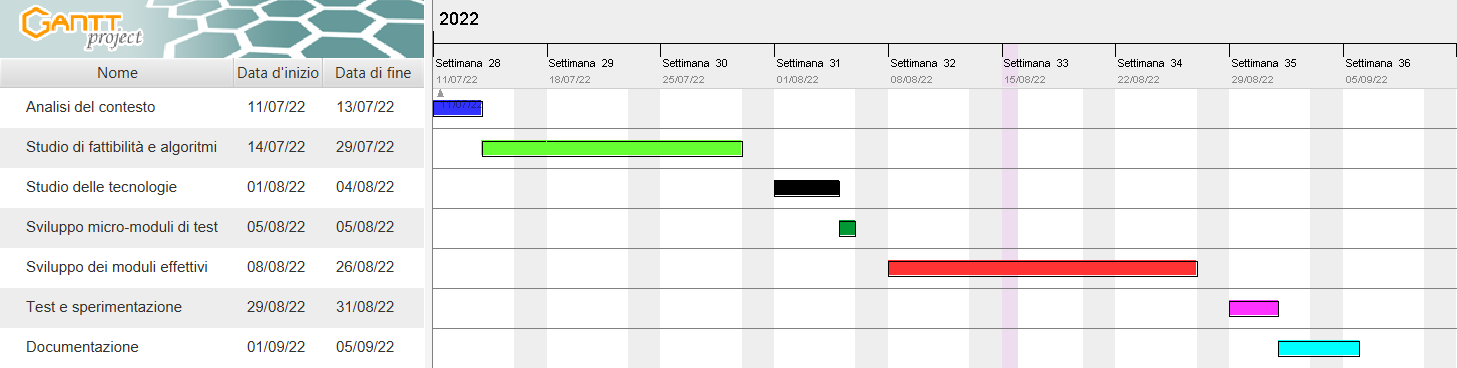
\includegraphics[width=0.95\columnwidth]{ganttdiagrams/Gantt Stage Ergon.png}
    \caption{Diagramma di \textit{Gantt} delle attività}
    \label{gantt-diagramma}
\end{figure}

%**************************************************************
\subsection{Analisi preventiva dei rischi}
\noindent Durante la fase iniziale dello \textit{stage}, sono stati rilevati dei possibili rischi che avrebbero potuto presentarsi
durante il percorso del progetto.\\
Si sono dunque trovate delle soluzioni che potessero arginare i problemi. In particolare:
\begin{enumerate}
    \item \textbf{Comprensione e confronto degli algoritmi}\\[0.2cm]
    \textbf{Problema:} il progetto richiede un'ampia fase di studio che riguarda principalmente la teoria
    delle tecniche per la risoluzione di problemi di \gls{ricercaoperativag} e Ottimizzazione Combinatoria.
    Questo può portare la possibilità di non comprendere fino in fondo l'algoritmo e può essere difficile cogliere e confrontare
    i pregi e difetti di ciascuno di essi.\\[0.2cm]
    \textbf{Soluzione:} è stato organizzato un incontro iniziale con il \textit{tutor}
    per fornire una base da cui poi iniziare una ricerca più approfondita.
    Sono state fornite anche delle dispense utili per rafforzare la base di partenza.
    \item \textbf{Tecnologie e ambiente di sviluppo}\\[0.2cm]
    \textbf{Problema:} sono richieste alcune tecnologie, come per esempio \textit{\gls{entityframeworkg}} $^{[g]}$ o
    \textit{\gls{devexpressg}} a me assolutamente ignote.
    Sebbene avessi delle basi abbastanza solide di \textit{C\#} derivanti dalla conoscenza di altri linguaggi
    quali \textit{\gls{C++g}} $^{[g]}$ e \textit{\gls{javag}} $^{[g]}$, venivano richieste tuttavia
    alcune tecnologie integrate nel linguaggio, come per esempio le \textit{\gls{linqg}} $^{[g]}$ (\textit{Language-Integrated Query}), anch'esse ignote. L'ambiente di sviluppo e
    l'\textit{\gls{ideg}} $^{[g]}$ non erano mai stati utilizzati.\\[0.2cm]
    \textbf{Soluzione:} sono stati forniti dei riferimenti consigliati per l'autoapprendimento.
    Tuttavia qualsiasi dubbio ulteriore
    poteva essere richiesto al \textit{tutor}. È stato effettuato insieme al \textit{tutor} il \textit{setup} dell'ambiente di sviluppo e la conseguente creazione dei \textit{\gls{databaseg}} $^{[g]}$.
    \item \textbf{Calibrazione dei parametri e funzione di valutazione}\\[0.2cm]
    \textbf{Problema:} dopo la scelta e l'implementazione dell'algoritmo, è molto importante:
    \begin{itemize}
        \item definire una funzione di valutazione che vada a descrivere in maniera "buona" l'andamento dell'algoritmo stesso;
        \item calibrare i parametri in base allo spazio delle soluzioni del problema preso in esame.
    \end{itemize}
    Entrambe sono azioni molto delicate che possono compromettere il funzionamento stesso dell'algoritmo anche
    se implementato correttamente.\\[0.2cm]
    \textbf{Soluzione:} cercare una costruzione e calibrazione per passi e presentarle in una discussione con il \textit{tutor},
    in modo tale da creare una \textit{baseline} su cui basarsi per continuare con i passi successivi.

\end{enumerate}

\noindent
%**************************************************************
\section{Organizzazione del testo}
\noindent Di seguito viene illustrata l'organizzazione dei capitoli successivi:
\begin{description}
    \item[{\hyperref[cap:studio-fattibilita]{Il secondo capitolo}}] 
    approfondisce lo studio di fattibilità effettuato, utile per entrare a conoscenza
    delle più utilizzate tecniche di Ottimizzazione Combinatoria e per analizzare
    quali siano i vantaggi e svantaggi di ognuna di esse.
    
    \item[{\hyperref[cap:analisi-requisiti]{Il terzo capitolo}}]
    descrive l'analisi dei requisiti del progetto, comprensiva di diagrammi dei
    casi d'uso e raccolta dei requisiti derivanti dall'analisi di questi ultimi.
    
    \item[{\hyperref[cap:progettazione-codifica]{Il quarto capitolo}}]
    approfondisce le fasi di progettazione e codifica, comprensiva di diagrammi delle classi
    e di approfondimenti a livello implementativo.
    
    \item[{\hyperref[cap:verifica-validazione]{Il quinto capitolo}}]
    espone tutte le verifiche effettuate durante il progetto e la validazione
    finale a conferma dei requisiti inizialmente stilati nella fase di
    analisi dei requisiti.
    
    \item[{\hyperref[cap:conclusioni]{Il sesto capitolo}}]
    presenta le conclusioni tratte dallo \textit{stage}, comprensivo di conoscenze
    acquisite e considerazioni di carattere personale.
\end{description}             % Introduzione
% !TEX encoding = UTF-8
% !TEX TS-program = pdflatex
% !TEX root = ../tesi.tex

%**************************************************************
\newgeometry{a4paper, left=30mm, right=30mm, top=5mm, bottom=30mm}
\chapter{Studio di fattibilità}
\label{cap:studio-fattibilita}
%**************************************************************

\noindent \intro{In questo capitolo viene esposto lo studio di fattibilità,
in cui verranno evidenziati i punti critici, i vantaggi e gli svantaggi delle
soluzioni analizzate.}\\

%**************************************************************
\section{Introduzione allo studio}
\noindent Lo studio di fattibilità rappresenta una delle parti più corpose
del progetto in quanto viene richiesto un ampio periodo di autoapprendimento
dei principali algoritmi di \gls{ricercaoperativag} e di Ottimizzazione Combinatoria,
seguito da un'ulteriore approfondimento attraverso la consultazione di vari \textit{paper}
disponibili \textit{online}.\\

\noindent Questa prima parte definirà una prima scelta tra gli algoritmi disponibili in base alle informazioni reperite.\\

\noindent La seconda parte invece consiste nello sviluppo di micro-moduli di \textit{test} sulle scelte effettuate
precedentemente, in modo tale da poter effettuare un'analisi e un confronto accurati basati su parametri che verranno
definiti successivamente.\\

\noindent Considerando anche il rapporto tra costi e risorse, le soluzioni che sono state identificate come le più plausibili e sottoposte a uno studio più approfondito sono:
\begin{enumerate}
    \item Algoritmo \textit{greedy}
    \item \textit{Tabu search}
    \item Algoritmo genetico
\end{enumerate}

\noindent Prima di proseguire con lo studio di fattibilità, è necessario dichiarare le metriche che sono state
utilizzate per effettuare un confronto equo tra gli algoritmi. Chiaramente, esse derivano dagli obiettivi che
l'algoritmo deve soddisfare per risolvere il problema.\\
Vengono elencati in seguito i parametri:
\begin{itemize}
    \item \textbf{Efficienza}: la capacità dell'algoritmo di utilizzare meno risorse di calcolo possibile per risolvere il problema;
    \item \textbf{Efficacia}: la capacità dell'algoritmo di risolvere il problema fornendo una soluzione il più possibile corretta;
    \item \textbf{Complessità implementativa}: quantitavo di risorse temporali impiegate per sviluppare l'algoritmo;
    \item \textbf{Paper}: dichiarazioni o dati di esperimenti già effettuati, come in \cite{siteA:paper-chen} \cite{siteR:paper-roli} \cite{siteU:paper-carlos}.
\end{itemize}

\newgeometry{a4paper, left=30mm, right=30mm, top=31mm, bottom=30mm}

%**************************************************************
\section{Soluzioni proposte}
\noindent Per ogni soluzione proposta, viene effettuata una breve introduzione, seguita da vantaggi e svantaggi.
Gli pseudocodici che descrivono in maniera sintetica i micro-moduli di \textit{test} si basano sul problema di \textit{string replacement}.
In questo problema, date una striga corretta e una errata entrambe di lunghezza $n$, il problema consiste nel correggere i caratteri della stringa errata
in modo tale da ottenere due stringhe uguali.
Si è volutamente scelto questo tipo di problema poichè sembrava sufficientemente semplice per poter prendere confidenza con gli algoritmi stessi.
Se i micro-moduli di \textit{test} fossero stati sviluppati intercalandoli all'interno del contesto del problema da risolvere, si avrebbe avuto un
enorme spreco di risorse temporali.

%**************************************************************
\subsection{Algoritmo \textit{Greedy}}
\noindent L'algoritmo \textit{greedy} ("\textit{goloso}") \cite{Cormen:algoritmi} viene così chiamato poichè basa la ricerca di una buona
soluzione \gls{ammissibileg} $^{[g]}$ sulla scelta, secondo un criterio predefinto, della miglior soluzione disponibile ad ogni passo, senza
rimettere in discussione la scelta appena effettuata.\\
Di seguito viene presentato lo pseudocodice dell'algoritmo \textit{greedy} per il problema in esame.

\begin{algorithm}[!h]
    \captionsetup{labelformat=empty}
    \caption{Pseudocodice \textit{string replacement} - Algoritmo \textit{greedy}}
    \vspace{0.1cm}
    \hspace*{\algorithmicindent} \textbf{\textit{Input}:} {$stringa\_corretta$}, {$stringa\_errata$}\\
    \hspace*{\algorithmicindent} \textbf{\textit{Output}:} {$funzione\_obiettivo$}
    \begin{algorithmic}[1]
        \Procedure{My\_Greedy\_Algorithm}{$stringa\_corretta$, $stringa\_errata$}
        \State {$array_{str\_err} \gets generate\_array(stringa\_errata)$}
        \State {$array_{str\_corr} \gets generate\_array(stringa\_corretta)$}
        \State {$funzione\_obiettivo \gets calcola\_fo(array_{str\_corr}$, $array_{str\_err})$}
        \State {$pos \gets 0$}
        \ForAll {$element \in array_{str\_err}$}
            \If {$element \neq array_{str\_corr}[pos]$}
                \State $element = array_{str\_corr}[pos]$
                \State {$funzione\_obiettivo \gets funzione\_obiettivo - 1$}
            \EndIf
            \State {$pos \gets pos + 1$}
        \EndFor
        \State \Return {$funzione\_obiettivo$}
        \EndProcedure
    \end{algorithmic}
\end{algorithm}

\noindent \paragraph{Osservazioni}\hfill\\
Come si può notare, l'algoritmo \textit{greedy} è molto intuitivo e, in questo caso,
anche banale.
Infatti, ad ogni iterazione, definiti $x$ come l'elemento in posizione $pos$ nella
stringa errata e $y$ come l'elemento, nella stessa posizione, nella stringa corretta,
se $x \neq y$, si effettua un replace di $x$ con la scelta migliore disponibile
in quel momento, ovvero $y$ stesso; se $x = y$, non è necessario effettuare alcuna operazione.

\noindent \paragraph{Aspetti positivi}
\begin{itemize}
    \item Bassa complessità implementativa;
    \item Bassa complessità computazionale dell'algoritmo;
    \item Possibilità di effettuare scelte \textit{greedy} differenti in problemi di vaste dimensioni.
\end{itemize}
\noindent \paragraph{Aspetti negativi}
\begin{itemize}
    \item Possibilmente inefficace, può non fornire una buona soluzione a causa
    delle scelte \textit{greedy} effettuate ad ogni iterazione che possono scartare soluzioni
    migliori nel lungo periodo.
\end{itemize}
%**************************************************************
\subsection{\textit{Tabu search}}
\noindent La \textit{Tabu search} \cite{siteS:dispense-de-giovanni} è un metodo, classificato come \textit{Trajectory Method} (\textit{Metodo a traiettoria}), basato su \gls{ricercalocaleg} $^{[g]}$
in grado di eludere l'intrappolamento del metodo in un minimo locale sfruttando costantemente la memoria.\\
La \gls{ricercalocaleg} si basa sull’idea di migliorare
una soluzione iniziale esplorandone un intorno
opportunamente definito. Se l’ottimizzazione
dell’intorno produce una soluzione migliorante,
il procedimento viene ripetuto
considerando come soluzione corrente la soluzione
appena determinata.
La \textit{Tabu search}, oltre a ricordare la migliore soluzione corrente, salva, in quella che viene definita \textit{Tabu list},
anche le {$k$} mosse precedentemente effettuate in modo tale da non incombere nel rischio di un ciclo nel breve periodo.\\
Viene dunque orientata la ricerca tramite la modifica del vicinato in funzione della storia dell'esplorazione, ma anche attraverso la diversificazione dei sottospazi
di ricerca tramite il passaggio per soluzioni non ammissibili.
L'algoritmo verrà descritto più approfonditamente nella Sezione §\hyperref[sec:tabu-search]{4.4}.\\
Di seguito viene presentato lo pseudocodice della \textit{Tabu search} per il problema in esame (rivisitazione dell'algoritmo proposto in \cite{siteO:solid-github}).\\
\begin{algorithm}[!h]
    \captionsetup{labelformat=empty}
    \caption{Pseudocodice \textit{string replacement} - \textit{Tabu search}}
    \vspace{0.1cm}
    \hspace*{\algorithmicindent} \textbf{\textit{Input}:} {$stringa\_corretta$}, {$stringa\_errata$}, {$capienza\_tabu\_list$}, {$max\_iterazioni$}\\
    \hspace*{\algorithmicindent} \textbf{\textit{Output}:} {$funzione\_obiettivo$}
    \begin{algorithmic}[1]
        \Procedure{My\_Tabu\_Search}{$stringa\_corretta$, $stringa\_errata$, $capienza\_tabu\_list$, $max\_iterazioni$}
        \State {$sol_{curr} \gets stringa\_errata$}
        \State {$funzione\_obiettivo_{curr} \gets stringa\_corretta.Length$}
        \State {$funzione\_obiettivo_{best} \gets funzione\_obiettivo_{curr}$}
        \State {$conta \gets 0$}
        \While {$conta < max\_iterazioni$}
            \State {$vicinato \gets genera\_vicinato()$}
            \While{$vicinato.Length > 0$ \textbf{and} $conta < max\_iterazioni$}
                \State {$vicino_{migl} \gets ottieni\_miglior\_vicino(vicinato)$}
                \If {$vicino_{migl} \not\in tabu\_list$}
                    \State {$funzione\_obiettivo_{curr} \gets calcola\_fo(vicino_{migl})$}
                    \If {$funzione\_obiettivo_{curr} < funzione\_obiettivo_{best}$}
                        \State Inserisci {$vicino_{migl}$} nella {$tabu\_list$} considerando la {$capienza\_tabu\_list$}
                        \State $sol_{curr} \gets vicino_{migl}$
                        \State {$funzione\_obiettivo_{best} \gets funzione\_obiettivo_{curr}$}
                        \State {$conta \gets conta + 1$}
                        \State {$\textbf{break}$}
                    \EndIf
                \EndIf
                \State Rimuovi {$vicino_{migl}$} dal {$vicinato$}
                \State {$conta \gets conta + 1$}
            \EndWhile
        \EndWhile
        \State \Return {$funzione\_obiettivo$}
        \EndProcedure
    \end{algorithmic}
\end{algorithm}
\vspace*{-0.4cm}
\noindent \paragraph{Osservazioni}\hfill\\
\noindent Notiamo come il ruolo della {$tabu\_list$} sia fondamentale in quanto, in caso di appartenza della mossa alla {$tabu\_list$}, non fa calcolare e
conseguentemente fare il confronto con {$funzione\_obiettivo_{best}$}. Inoltre, se la {$funzione\_obiettivo_{curr}$} non è migliorante, l'iterazione
viene comunque contata.\\
Di seguito vengono elencati i pro e i contro del seguente approccio (come descritto in \cite{siteQ:paper-lo-go} \cite{siteT:articolo-tabu-search}).\\
\noindent \paragraph{Aspetti positivi}
\begin{itemize}
    \item Bassa complessità implementativa;
    \item Bassa complessità computazionale dell'algoritmo;
    \item Velocità di raggiungimento del minimo locale;
    \item Fuga da ottimi locali.
\end{itemize}

\noindent \paragraph{Aspetti negativi}
\begin{itemize}
    \item Possibilmente inefficace, può non fornire una buona soluzione;
    \item Difficile calibrazione dei parametri;
    \item Numero di iterazioni necessario può essere molto alto;
    \item Necessità di una soluzione iniziale.
\end{itemize}
%**************************************************************
\subsection{Algoritmo genetico}
\noindent L'algoritmo genetico \cite{siteS:dispense-de-giovanni} è un metodo, classifcato come \textit{population based}, basato sul concetto che la natura
abbia la tendenza ad organizzarsi in strutture ottimizzate, in gran parte ispirato
alle teorie sull'evoluzione di \textit{Charles Darwin}.\\
\noindent In particolare, ad ogni iterazione, non viene mantenuta una sola soluzione, ma un insieme di soluzioni, definita anche come popolazione.
Gli individui (soluzioni) vengono codificati tramite un cromosoma contenente una serie di geni (variabili decisionali del problema) e, per
ogni individuo appartente alla popolazione, viene associata quella che viene definita come la sua idoneità, tramite l'utilizzo di una
funzione di \textit{fitness}, che guida il processo di selezione, basato su metodi probabilistici (es: \textit{metodo Montecarlo}, \textit{linear ranking}, \textit{torneo-n}).\\
Prima di ogni iterazione vengono dunque presi gli individui e verranno in seguito accoppiati tramite degli operatori di ricombinazione
(es: \textit{crossover uniforme}, \textit{cut-point crossover}, \textit{mutazione}...)
per generare dei figli che assumeranno le migliori caratteristiche dei genitori. Alla fine dell'algoritmo, verrà scelta la soluzione con la maggior \textit{fitness} possibile.\\
Di seguito viene presentato lo pseudocodice dell'algoritmo genetico per il problema in esame (rivisitazione dell'algoritmo proposto in \cite{siteO:solid-github}).
\vspace*{\fill}
\begin{algorithm}[!h]
    \captionsetup{labelformat=empty}
    \caption{Pseudocodice \textit{string replacement} - \textit{Algoritmo genetico}}
    \vspace{0.1cm}
    \hspace*{\algorithmicindent} \textbf{\textit{Input}:} {$stringa\_corretta$}, {$crossover\_rate$}, {$mutation\_rate$}, \\\hspace*{54pt}{$max\_iterazioni$}\\
    \hspace*{\algorithmicindent} \textbf{\textit{Output}:} {$sol_{best}, fitness_{best}$}
    \begin{algorithmic}[1]
        \Procedure{My\_Genetic\_Algorithm}{$stringa\_corretta$, \par$crossover\_rate$, $mutation\_rate$, $max\_iterazioni$}
        \State {$arr_{str\_corr} \gets codifica(stringa\_corretta)$}
        \State {$lista\_pop \gets inizializza\_pop()$}
        \State {$set\_fitness()$}
        \State {$fitness_{best} \gets most\_fitness\_val(arr_{str\_corr})$}
        \State {$sol_{best} \gets most\_fitness\_sol(arr_{str\_corr})$}
        \State {$num_{crossover} \gets calculate\_num\_crossover(crossover\_rate$, $lista\_pop)$}
        \State {$conta \gets 0$}
        \While {$conta < max\_iterazioni$}
        \State {$lista\_pop \gets seleziona\_individui(num_{crossover})$}
        \State {$set\_fitness()$}
            \State {$i \gets 0$}
        \algstore{part 1}
    \end{algorithmic}
\end{algorithm}
\vspace*{\fill}
\begin{algorithm}
    \begin{algorithmic}
        \algrestore{part 1}
            \While {$i < num_{crossover}$}
                \State {$lista\_genitori \gets seleziona\_individui(2)$}
                \State {$figlio \gets genera\_figlio(lista\_genitori)$}
                \State Aggiungi il {$figlio$} in coda alla lista {$nuova\_pop$}
                \State {$i \gets i + 1$}
            \EndWhile
            \State {$lista\_pop \gets nuova\_pop$}
            \State {$lista\_pop \gets mutazione\_rand(lista\_pop)$}
            \State {$set\_fitness()$}
            \State {$fitness_{curr} \gets most\_fitness\_val(arr_{str\_corr})$}
            \State {$sol_{curr} \gets most\_fitness\_sol(arr_{str\_corr})$}
            \If {$fitness_{curr} > fitness_{best}$}
                \State {$fitness_{best} \gets fitness_{curr}$}
                \State {$sol_{best} \gets sol_{curr}$}
            \EndIf
            \State {$conta \gets conta + 1$}
        \EndWhile
        \State \Return {$sol_{best}$, $fitness_{best}$}
        \EndProcedure
    \end{algorithmic}
\end{algorithm}

\noindent \paragraph{Osservazioni}\hfill\\
Si noti come, per ogni popolazione, vengano scelti un numero di individui dipendente dal {$crossover\_rate$}
e vengano effettuati {$num_{crossover}$} \textit{crossover} scegliendo 2 individui dalla popolazione che fungono da genitori.
Viene dunque creata una nuova popolazione di figli a cui viene anche applicata una mutazione a un figlio \textit{random} per
variare il patrimonio genetico, in modo tale da avere più possibilità di trovare buone caratteristiche.\\
Di seguito vengono elencati i pro e i contro del seguente approccio (come riportato in \cite{siteP:articolo-alg-gen} \cite{siteQ:paper-lo-go}).\\

\noindent \paragraph{Aspetti positivi}
\begin{itemize}
    \item Fuga da ottimi locali;
    \item Analisi di più sottospazi delle soluzioni, grazie alla varietà della popolazione.
    \item possibilità di esplorare facilmente diverse aree dello spazio di ricerca, grazie a componenti stocastiche
\end{itemize}

\noindent \paragraph{Aspetti negativi}
\begin{itemize}
    \item Modesta complessità implementativa;
    \item Possibilmente inefficace, può non fornire una buona soluzione;
    \item Difficile calibrazione dei parametri per la forte presenza di componenti stocastiche;
    \item Difficile codifica degli individui in alcuni problemi;
    \item Numero di iterazioni necessario può essere molto alto.
\end{itemize}
\newpage
%**************************************************************
\section{Conclusioni dello studio}
\label{conclusione-studio-fattibilita}
\noindent Lo studio è servito per capire come funzionassero gli algoritmi e quali fossero i loro pregi e difetti.
Di seguito si hanno i risultati dell'analisi dei 3 algoritmi eseguiti singolarmente su una singola istanza.\\
\\
\noindent \textbf{Input degli algoritmi}
\begin{itemize}
    \item Algoritmo \textit{greedy}:
    \begin{itemize}
        \item \textbf{stringa corretta:} \textit{tabusearch};
        \item \textbf{stringa errata:} \textit{correctnot}.
    \end{itemize}
    \item \textit{Tabu search}:
    \begin{itemize}
        \item \textbf{stringa corretta:} \textit{tabusearch};
        \item \textbf{stringa errata:} \textit{correctnot};
        \item \textbf{capienza tabu list:} 50;
        \item \textbf{massimo numero di iterazioni:} 500.
    \end{itemize}
    \item Algoritmo \textit{greedy}:
    \begin{itemize}
        \item \textbf{stringa corretta:} \textit{tabusearch};
        \item \textbf{\textit{crossover rate}:} 0.5;
        \item \textbf{\textit{mutation rate}:} 0.7;
        \item \textbf{massimo numero di iterazioni:} 500.
    \end{itemize}
\end{itemize}

\renewcommand{\arraystretch}{1.6}

% tabella con i risultati
\begin{center}
    \begin{longtable}{|m{3cm}|m{3cm}|m{3cm}|m{3cm}|}
    \caption{Tabella dei risultati medi dell'analisi degli algoritmi dopo 10 esecuzioni}
    \label{tab:risultati-studio-fattibilita}
    \\ \hline
    \centering \textbf{Tipologia} & \centering \textbf{Efficacia (\%)} & \centering \textbf{Efficienza (ms)} & \centering \textbf{Tempo di realizzazione (h)} \arraybackslash \\
    \hline
    \centering Algoritmo \textit{greedy} & \centering 100 & \centering 0,45 & \centering 0,5 \arraybackslash \\
    \hline
    \centering \textit{Tabu search} & \centering 98 & \centering 1289,76 & \centering 2,5 \arraybackslash \\
    \hline
    \centering Algortimo Genetico & \centering 92 & \centering 5127,24 & \centering 5 \arraybackslash \\
    \hline
    \end{longtable}
\end{center}%

dove:
\begin{itemize}
    \item LC = lettere corrette
    \item LT = lettere totali
    \item Efficacia = $10 \cdot \sum_{i=1} ^{10}{\frac{LC_i}{LT_i}}$\\
\end{itemize}
\noindent Dai risultati dell'istanza descritta in precedenza, l'algoritmo \textit{greedy} potrebbe risultare
il più efficiente ed efficace,
ma per il problema che si andrà a risolvere non può essere considerato
molto soddisfacente, in quanto le scelte
non vengono mai rimesse in discussione e potrebbero dunque escludere soluzioni potenzialmente migliori
(esempio nella Sezione §\ref{sec:descrizione-stage-intro}).\\
Si può notare, inoltre, come l'algoritmo genetico, sebbene sia interessante per il mantenimento di più soluzioni ad ogni iterazione,
abbia richiesto più tempo per essere implementato. Si è deciso di scartarlo perchè si sarebbe corso il rischio di lasciare il lavoro incompleto,
non portando dunque a termine gli obiettivi obbligatori dello \textit{stage} descritti nella Sezione §\ref{sec:obiettivi}.\\
La \textit{Tabu search}, in base anche all'esperienza maturata attraverso lo studio, sembrerebbe rappresentare un buon compromesso sia a livello
di efficacia ed efficienza che a livello implementativo (come descritto anche in \cite{siteS:dispense-de-giovanni}).
Per quanto riguarda la soluzione iniziale, questa potrebbe essere generata a partire da un algoritmo \textit{greedy},
data la sua bassa complessità computazionale. In questo modo sarebbe possibile avere già a disposizione una buona soluzione di base.\\             % Studio di fattibilità
% !TEX encoding = UTF-8
% !TEX TS-program = pdflatex
% !TEX root = ../tesi.tex

%**************************************************************
\chapter{Analisi dei requisiti}
\label{cap:analisi-requisiti}
%**************************************************************

\noindent \intro{Breve introduzione al capitolo}\\

\section{Casi d'uso}

\noindent Per lo studio dei casi di utilizzo del prodotto sono stati creati dei diagrammi.
I diagrammi dei casi d'uso (in inglese \emph{Use Case Diagram}) sono diagrammi di tipo \gls{umlg} dedicati alla descrizione delle funzioni o servizi offerti da un sistema, così come sono percepiti e utilizzati dagli attori che interagiscono col sistema stesso.
Essendo il progetto finalizzato alla creazione di un tool per l'automazione di un processo, le interazioni da parte dell'utilizzatore devono essere ovviamente ridotte allo stretto necessario. Per questo motivo i diagrammi dei casi d'uso risultano semplici e in numero ridotto.\\

\noindent A livello formale, i diagrammi dei casi d'uso avranno la seguente forma:
\begin{center}
    \textbf{UC<CodicePadre>.<CodiceFiglio>}
\end{center}
\noindent È importante ribadire come questo formalismo sia gerarchico, ovvero un codice figlio
può essere codice padre di un suo eventuale codice figlio. Possono essere figli le generalizzazioni e i sottocasi d'uso.\\

\noindent Nella figura di seguito verrà illustrato il diagramma del sistema principale con tutti i casi d'uso.
\begin{figure}[!h] 
   \centering 
   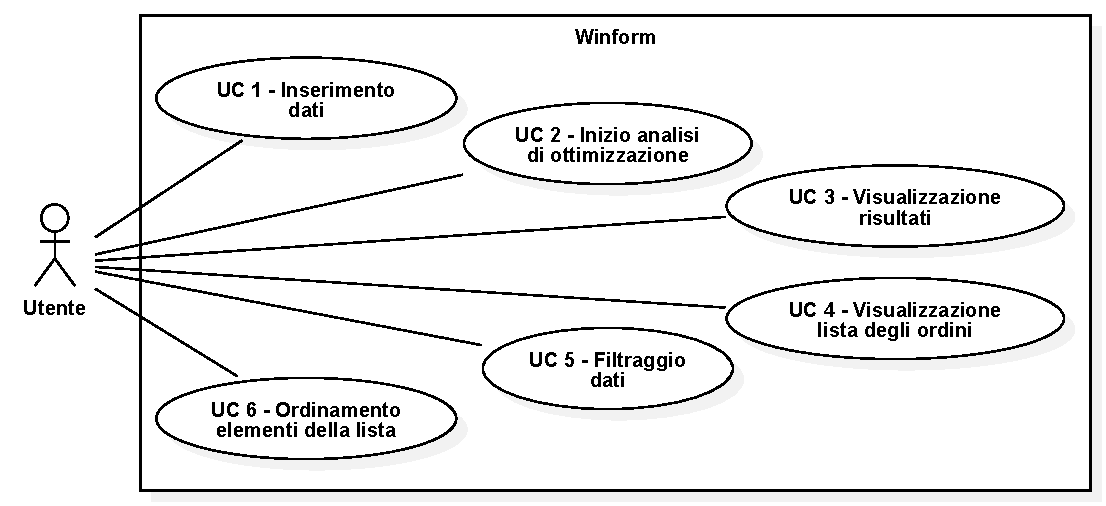
\includegraphics[width=0.95\columnwidth]{usecase/winform.pdf} 
   \caption{Use case - sistema principale}
\end{figure}

\noindent \textbf{\large UC 1 - Inserimento dati}
\label{uc:inserimento-dati}
\begin{figure}[!h] 
    \centering 
    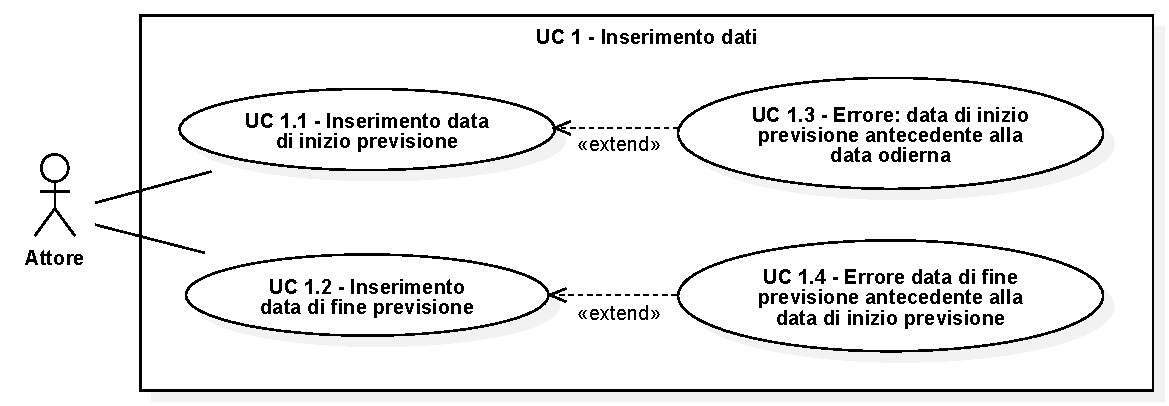
\includegraphics[width=0.95\columnwidth]{usecase/UC 1.pdf} 
    \caption{UC1 - Inserimento dati}
\end{figure}
\begin{itemize}

	\item \textbf{Attori primari: }
		\begin{itemize}
			\item Utente.
		\end{itemize}

	\item \textbf{Precondizione: }\\[0.3cm]
		L'utente è dentro la \textit{form} e non ha ancora inserito alcun dato.

	\item \textbf{Scenario principale: }
		\begin{enumerate}
			\item L'utente inserisce i dati.
		\end{enumerate}
		

	\item \textbf{Postcondizione: }\\[0.3cm]
		L'utente ha inserito i dati correttamente.

\end{itemize}

\vspace{0.4cm}

\noindent \textbf{\large UC 1.1 - Inserimento data di inizio previsione}
\label{uc:inserimento-data-inizio-prev}
\begin{itemize}

	\item \textbf{Attori primari: }
		\begin{itemize}
			\item Utente.
		\end{itemize}

	\item \textbf{Precondizione: }\\[0.3cm]
		L'utente è dentro la \textit{form} e non ha ancora inserito la data di inizio previsione.

	\item \textbf{Scenario principale: }
		\begin{enumerate}
			\item L'utente seleziona la data di inizio previsione.
		\end{enumerate}

	\item \textbf{Postcondizione: }\\[0.3cm]
		L'utente ha inserito la data di inizio previsione correttamente.

	\item \textbf{Scenario alternativo: }
		\begin{itemize}
		    \item La \textit{form} segnala un errore di immissione dati (\hyperref[uc:err-inserimento-data-inizio-prev]{UC 1.3}).
		\end{itemize}

\end{itemize}

\vspace{0.4cm}


\newpage

\noindent \textbf{\large UC 1.2 - Inserimento data di fine previsione}
\label{uc:inserimento-data-fine-prev}
\begin{itemize}

	\item \textbf{Attori primari: }
		\begin{itemize}
			\item Utente.
		\end{itemize}

	\item \textbf{Precondizione: }\\[0.3cm]
		L'utente è dentro la \textit{form} e non ha ancora inserito la data di fine previsione.

	\item \textbf{Scenario principale: }
		\begin{enumerate}
			\item L'utente inserisce la data di fine previsione;
		\end{enumerate}

	\item \textbf{Postcondizione: }\\[0.3cm]
		L'utente ha inserito la data di fine previsione correttamente.

	\item \textbf{Scenario alternativo: }
		\begin{itemize}
		    \item La \textit{form} segnala un errore di immissione dati (\hyperref[uc:err-inserimento-data-fine-prev]{UC 1.4}).
		\end{itemize}

\end{itemize}

\vspace{0.4cm}

\noindent \textbf{\large UC 1.3 - Errore: data di inizio previsione antecedente alla data odierna}
\label{uc:err-inserimento-data-inizio-prev}
\begin{itemize}

	\item \textbf{Attori primari: }
		\begin{itemize}
			\item Utente.
		\end{itemize}

	\item \textbf{Precondizione: }\\[0.3cm]
		L'utente è dentro la \textit{form} e ha inserito una data di inizio previsione antecedente
		alla data odierna.

	\item \textbf{Scenario principale: }
		\begin{enumerate}
			\item L'utente conferma la data di inizio previsione;
			\item L'utente visualizza un errore generato dalla \textit{form}.
		\end{enumerate}
		

	\item \textbf{Postcondizione: }\\[0.3cm]
		L'utente viene avvisato dell'errore di immissione.

\end{itemize}

\vspace{0.4cm}

\noindent \textbf{\large UC 1.4 - Errore: data di fine previsione antecedente alla data di \\\hspace*{56pt}inizio previsione}
\label{uc:err-inserimento-data-fine-prev}
\begin{itemize}

	\item \textbf{Attori primari: }
		\begin{itemize}
			\item Utente.
		\end{itemize}

	\item \textbf{Precondizione: }\\[0.3cm]
		L'utente è dentro la \textit{form} e ha inserito una data di fine previsione antecedente
		alla data odierna.

	\item \textbf{Scenario principale: }
		\begin{enumerate}
			\item L'utente conferma la data di fine previsione;
			\item L'utente visualizza un errore generato dalla \textit{form}.
		\end{enumerate}
		

	\item \textbf{Postcondizione: }\\[0.3cm]
		L'utente viene avvisato dell'errore di immissione.

\end{itemize}

\vspace{0.4cm}

\noindent \textbf{\large UC 2 - Inizio analisi di ottimizzazione}
\label{uc:inizio-analisi-ottimizzazione}
\begin{itemize}

	\item \textbf{Attori primari: }
		\begin{itemize}
			\item Utente.
		\end{itemize}

	\item \textbf{Precondizione: }\\[0.3cm]
		L'utente è dentro la \textit{form} e ha inserito una data di inizio e fine previsione valide.

	\item \textbf{Scenario principale: }
		\begin{enumerate}
			\item L'utente conferma l'inizio dell'analisi di ottimizzazione.
		\end{enumerate}
		

	\item \textbf{Postcondizione: }\\[0.3cm]
		L'utente ha effettuato l'analisi di ottimizzazione per le date di inizio e fine previsione e visualizza correttamente i
		risultati (\hyperref[uc:visualizzazione-risultati]{UC 3}).

\end{itemize}

\vspace{0.4cm}

\noindent \textbf{\large UC 3 - Visualizzazione risultati}
\label{uc:visualizzazione-risultati}
\begin{figure}[!h] 
    \centering 
    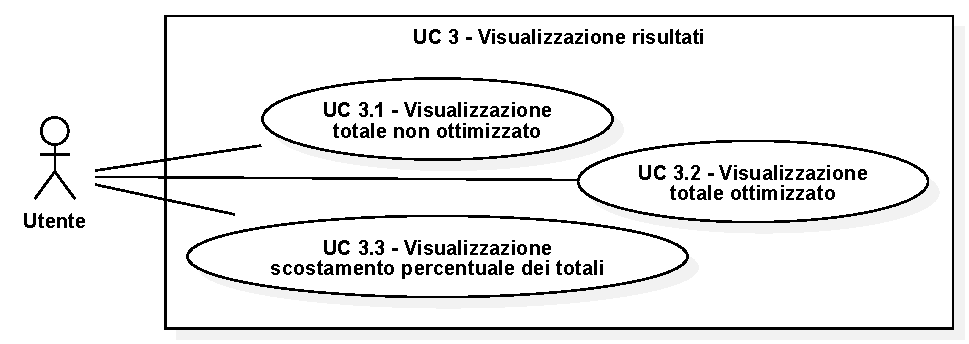
\includegraphics[width=0.95\columnwidth]{usecase/UC 3.pdf} 
    \caption{UC3 - Visualizzazione risultati}
\end{figure}
\begin{itemize}

	\item \textbf{Attori primari: }
		\begin{itemize}
			\item Utente.
		\end{itemize}

	\item \textbf{Precondizione: }\\[0.3cm]
		L'utente è dentro la \textit{form} e ha effettuato l'analisi di ottimizzazione correttamente.

	\item \textbf{Scenario principale: }
		\begin{enumerate}
			\item L'utente visualizza il totale non ottimizzato (\hyperref[uc:visualizzazione-totale-non-ottimizzato]{UC 3.1});
			\item L'utente visualizza il totale ottimizzato (\hyperref[uc:visualizzazione-totale-ottimizzato]{UC 3.2});
			\item L'utente visualizza lo scostamento percentuale dei totali (\hyperref[uc:visualizzazione-scostamento-percentuale-totali]{UC 3.3}).
		\end{enumerate}
		

	\item \textbf{Postcondizione: }\\[0.3cm]
		L'utente visualizza correttamente tutti i risultati.

\end{itemize}

\vspace{0.4cm}

\newpage

\noindent \textbf{\large UC 3.1 - Visualizzazione totale non ottimizzato}
\label{uc:visualizzazione-totale-non-ottimizzato}
\begin{itemize}

	\item \textbf{Attori primari: }
		\begin{itemize}
			\item Utente.
		\end{itemize}

	\item \textbf{Precondizione: }\\[0.3cm]
		L'utente è dentro la \textit{form} e ha effettuato l'analisi di ottimizzazione correttamente.

	\item \textbf{Scenario principale: }
		\begin{enumerate}
			\item L'utente visualizza il totale non ottimizzato.
		\end{enumerate}
		

	\item \textbf{Postcondizione: }\\[0.3cm]
		L'utente visualizza correttamente il totale non ottimizzato.

\end{itemize}

\vspace{0.4cm}

\noindent \textbf{\large UC 3.2 - Visualizzazione totale ottimizzato}
\label{uc:visualizzazione-totale-ottimizzato}
\begin{itemize}

	\item \textbf{Attori primari: }
		\begin{itemize}
			\item Utente.
		\end{itemize}

	\item \textbf{Precondizione: }\\[0.3cm]
		L'utente è dentro la \textit{form} e ha effettuato l'analisi di ottimizzazione correttamente.

	\item \textbf{Scenario principale: }
		\begin{enumerate}
			\item L'utente visualizza il totale ottimizzato.
		\end{enumerate}
		

	\item \textbf{Postcondizione: }\\[0.3cm]
		L'utente visualizza correttamente il totale ottimizzato.

\end{itemize}

\vspace{0.4cm}

\noindent \textbf{\large UC 3.3 - Visualizzazione scostamento percentuale dei totali}
\label{uc:visualizzazione-scostamento-percentuale-totali}
\begin{itemize}

	\item \textbf{Attori primari: }
		\begin{itemize}
			\item Utente.
		\end{itemize}

	\item \textbf{Precondizione: }\\[0.3cm]
		L'utente è dentro la \textit{form} e ha effettuato l'analisi di ottimizzazione correttamente.

	\item \textbf{Scenario principale: }
		\begin{enumerate}
			\item L'utente visualizza lo scostamento percentuale dei totali.
		\end{enumerate}
		

	\item \textbf{Postcondizione: }\\[0.3cm]
		L'utente visualizza correttamente lo scostamento percentuale dei totali.

\end{itemize}

\vspace{0.4cm}

\newpage

\noindent \textbf{\large UC 4 - Visualizzazione lista degli ordini}
\begin{figure}[!h] 
    \centering 
    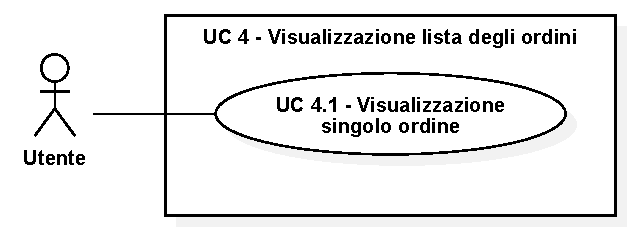
\includegraphics[width=0.65\columnwidth]{usecase/UC 4.pdf} 
    \caption{UC4 - Visualizzazione lista degli ordini}
\end{figure}
\label{uc:visualizzazione-lista-ordini}
\begin{itemize}

	\item \textbf{Attori primari: }
		\begin{itemize}
			\item Utente.
		\end{itemize}

	\item \textbf{Precondizione: }\\[0.3cm]
		L'utente è dentro la \textit{form} e ha effettuato l'analisi di ottimizzazione correttamente.

	\item \textbf{Scenario principale: }
		\begin{enumerate}
			\item L'utente visualizza la lista degli ordini da effettuare.
		\end{enumerate}
		

	\item \textbf{Postcondizione: }\\[0.3cm]
		L'utente visualizza correttamente la lista degli ordini da effettuare.

\end{itemize}

\vspace{0.4cm}

\vspace*{\fill}

\noindent \textbf{\large UC 4.1 - Visualizzazione singolo ordine}
\begin{figure}[!h] 
    \centering 
    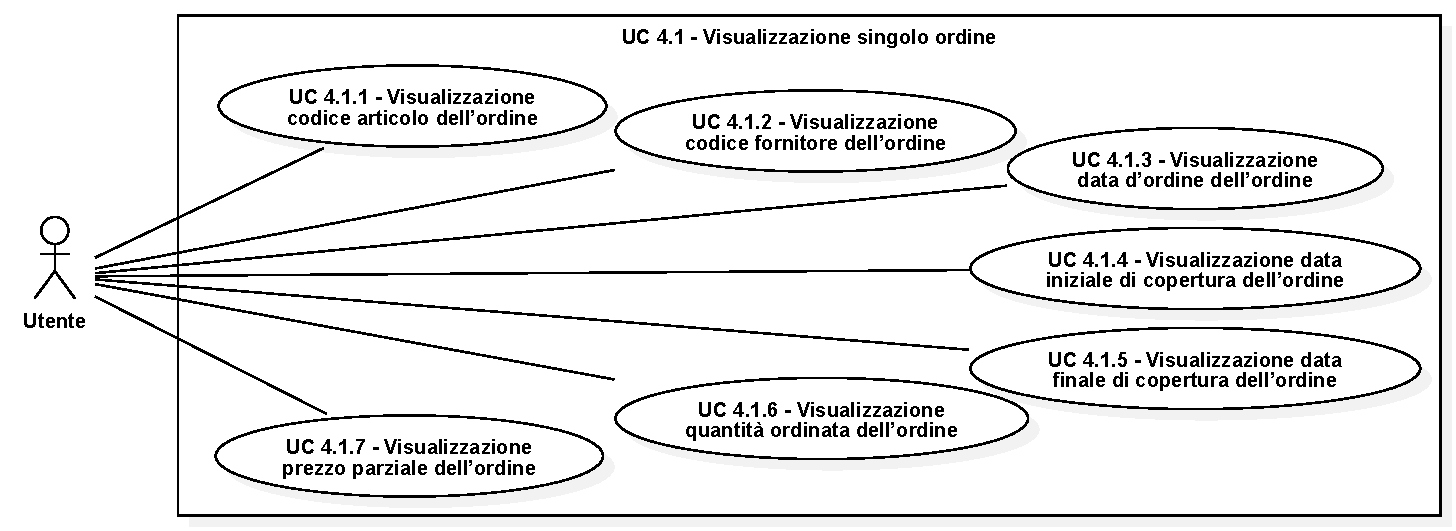
\includegraphics[width=0.95\columnwidth]{usecase/UC 4.1.pdf} 
    \caption{UC4.1 - Visualizzazione singolo ordine}
\end{figure}
\label{uc:visualizzazione-singolo-ordine}
\begin{itemize}

	\item \textbf{Attori primari: }
		\begin{itemize}
			\item Utente.
		\end{itemize}

	\item \textbf{Precondizione: }\\[0.3cm]
		L'utente visualizza correttamente la lista degli ordini.
		
	\vspace*{\fill}

		\newpage
	
	\item \textbf{Scenario principale: }
		\begin{enumerate}
			\item L'utente visualizza il singolo ordine con tutte le informazioni tra cui:
			\begin{itemize}
				\item codice articolo (\hyperref[uc:visualizzazione-codice-articolo]{UC 4.1.1});
				\item codice fornitore (\hyperref[uc:visualizzazione-codice-fornitore]{UC 4.1.2});
				\item data d'ordine (\hyperref[uc:visualizzazione-data-ordine]{UC 4.1.3});
				\item data iniziale di copertura (\hyperref[uc:visualizzazione-data-iniziale-copertura]{UC 4.1.4});
				\item data finale di copertura (\hyperref[uc:visualizzazione-data-finale-copertura]{UC 4.1.5});
				\item quantità ordinata (\hyperref[uc:visualizzazione-quantita-ordinata]{UC 4.1.6});
				\item prezzo parziale (\hyperref[uc:visualizzazione-prezzo-parziale-ord]{UC 4.1.7});
			\end{itemize}.
		\end{enumerate}
		

	\item \textbf{Postcondizione: }\\[0.3cm]
		L'utente visualizza correttamente il singolo ordine.

\end{itemize}

\vspace{0.4cm}

\noindent \textbf{\large UC 4.1.1 - Visualizzazione codice articolo dell'ordine}
\label{uc:visualizzazione-codice-articolo}
\begin{itemize}

	\item \textbf{Attori primari: }
		\begin{itemize}
			\item Utente.
		\end{itemize}

	\item \textbf{Precondizione: }\\[0.3cm]
		L'utente visualizza correttamente il singolo ordine.

	\item \textbf{Scenario principale: }
		\begin{enumerate}
			\item L'utente visualizza il codice articolo del singolo ordine.
		\end{enumerate}
		

	\item \textbf{Postcondizione: }\\[0.3cm]
		L'utente visualizza correttamente il codice articolo del singolo ordine.

\end{itemize}

\vspace{0.4cm}

\noindent \textbf{\large UC 4.1.2 - Visualizzazione codice fornitore dell'ordine}
\label{uc:visualizzazione-codice-fornitore}
\begin{itemize}

	\item \textbf{Attori primari: }
		\begin{itemize}
			\item Utente.
		\end{itemize}

	\item \textbf{Precondizione: }\\[0.3cm]
		L'utente visualizza correttamente il singolo ordine.

	\item \textbf{Scenario principale: }
		\begin{enumerate}
			\item L'utente visualizza il codice fornitore del singolo ordine.
		\end{enumerate}
		

	\item \textbf{Postcondizione: }\\[0.3cm]
		L'utente visualizza correttamente il codice fornitore del singolo ordine.

\end{itemize}

\vspace{0.4cm}

\newpage

\noindent \textbf{\large UC 4.1.3 - Visualizzazione data d'ordine dell'ordine}
\label{uc:visualizzazione-data-ordine}
\begin{itemize}

	\item \textbf{Attori primari: }
		\begin{itemize}
			\item Utente.
		\end{itemize}

	\item \textbf{Precondizione: }\\[0.3cm]
		L'utente visualizza correttamente il singolo ordine.

	\item \textbf{Scenario principale: }
		\begin{enumerate}
			\item L'utente visualizza la data d'ordine del singolo ordine.
		\end{enumerate}
		

	\item \textbf{Postcondizione: }\\[0.3cm]
		L'utente visualizza correttamente la data d'ordine del singolo ordine.

\end{itemize}

\vspace{0.4cm}

\noindent \textbf{\large UC 4.1.4 - Visualizzazione data iniziale di copertura dell'ordine}
\label{uc:visualizzazione-data-iniziale-copertura}
\begin{itemize}

	\item \textbf{Attori primari: }
		\begin{itemize}
			\item Utente.
		\end{itemize}

	\item \textbf{Precondizione: }\\[0.3cm]
		L'utente visualizza correttamente il singolo ordine.

	\item \textbf{Scenario principale: }
		\begin{enumerate}
			\item L'utente visualizza la data iniziale di copertura del singolo ordine.
		\end{enumerate}
		

	\item \textbf{Postcondizione: }\\[0.3cm]
		L'utente visualizza correttamente la data iniziale di copertura del singolo ordine.

\end{itemize}

\vspace{0.4cm}

\noindent \textbf{\large UC 4.1.5 - Visualizzazione data finale di copertura dell'ordine}
\label{uc:visualizzazione-data-finale-copertura}
\begin{itemize}

	\item \textbf{Attori primari: }
		\begin{itemize}
			\item Utente.
		\end{itemize}

	\item \textbf{Precondizione: }\\[0.3cm]
		L'utente visualizza correttamente il singolo ordine.

	\item \textbf{Scenario principale: }
		\begin{enumerate}
			\item L'utente visualizza la data finale di copertura del singolo ordine.
		\end{enumerate}
		

	\item \textbf{Postcondizione: }\\[0.3cm]
		L'utente visualizza correttamente la data finale di copertura del singolo ordine.

\end{itemize}

\vspace{0.4cm}

\newpage

\noindent \textbf{\large UC 4.1.6 - Visualizzazione quantità ordinata dell'ordine}
\label{uc:visualizzazione-quantita-ordinata}
\begin{itemize}

	\item \textbf{Attori primari: }
		\begin{itemize}
			\item Utente.
		\end{itemize}

	\item \textbf{Precondizione: }\\[0.3cm]
		L'utente visualizza correttamente il singolo ordine.

	\item \textbf{Scenario principale: }
		\begin{enumerate}
			\item L'utente visualizza la quantità ordinata del singolo ordine.
		\end{enumerate}
		

	\item \textbf{Postcondizione: }\\[0.3cm]
		L'utente visualizza correttamente la quantità ordinata del singolo ordine.

\end{itemize}

\vspace{0.4cm}

\noindent \textbf{\large UC 4.1.7 - Visualizzazione prezzo parziale dell'ordine}
\label{uc:visualizzazione-prezzo-parziale-ord}
\begin{itemize}

	\item \textbf{Attori primari: }
		\begin{itemize}
			\item Utente.
		\end{itemize}

	\item \textbf{Precondizione: }\\[0.3cm]
		L'utente visualizza correttamente il singolo ordine.

	\item \textbf{Scenario principale: }
		\begin{enumerate}
			\item L'utente visualizza il prezzo parziale del singolo ordine.
		\end{enumerate}
		

	\item \textbf{Postcondizione: }\\[0.3cm]
		L'utente visualizza correttamente il prezzo parziale del singolo ordine.

\end{itemize}

\vspace{0.4cm}

\noindent \textbf{\large UC 5 - Filtraggio dati}
\label{uc:filtraggio-dati}
\begin{figure}[!h] 
    \centering 
    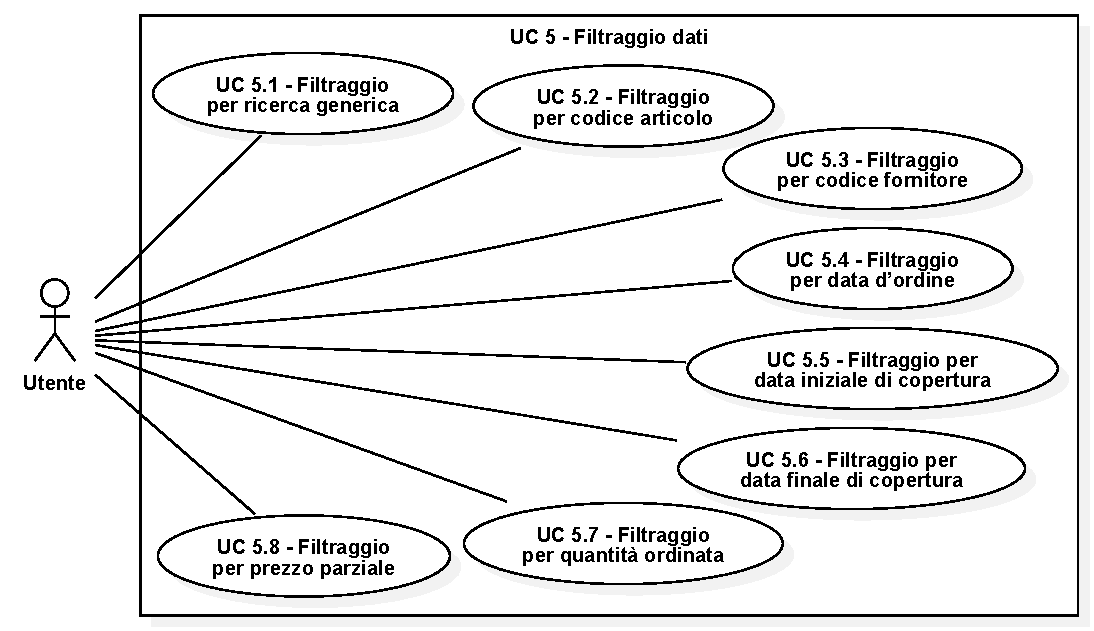
\includegraphics[width=0.95\columnwidth]{usecase/UC 5.pdf} 
    \caption{UC 5 - Filtraggio dati}
\end{figure}
\begin{itemize}

	\item \textbf{Attori primari: }
		\begin{itemize}
			\item Utente.
		\end{itemize}

	\item \textbf{Precondizione: }\\[0.3cm]
		L'utente visualizza correttamente la lista degli ordini.

	\item \textbf{Scenario principale: }
		\begin{enumerate}
			\item L'utente sceglie uno o più filtri da applicare alla lista.\\
			In particolare le tipologie di filtro disponibili sono per:
			\begin{itemize}
				\item codice articolo (\hyperref[uc:filtraggio-codice-articolo]{UC 5.1});
				\item codice articolo (\hyperref[uc:filtraggio-codice-articolo]{UC 5.2});
				\item codice fornitore (\hyperref[uc:filtraggio-codice-fornitore]{UC 5.3});
				\item data d'ordine (\hyperref[uc:filtraggio-data-ordine]{UC 5.4});
				\item data iniziale di copertura (\hyperref[uc:filtraggio-data-iniziale-copertura]{UC 5.5});
				\item data finale di copertura (\hyperref[uc:filtraggio-data-finale-copertura]{UC 5.6});
				\item quantità ordinata (\hyperref[uc:filtraggio-quantita-ordinata]{UC 5.7});
				\item prezzo parziale (\hyperref[uc:filtraggio-prezzo-parziale-ord]{UC 5.8});
			\end{itemize}
		\end{enumerate}
		

	\item \textbf{Postcondizione: }\\[0.3cm]
		L'utente visualizza correttamente tutti gli elementi che soddisfano i filtri applicati.

\end{itemize}

\vspace{0.4cm}

\noindent \textbf{\large UC 5.1 - Filtraggio per ricerca generica}
\label{uc:filtraggio-ricerca-generica}
\begin{itemize}

	\item \textbf{Attori primari: }
		\begin{itemize}
			\item Utente.
		\end{itemize}

	\item \textbf{Precondizione: }\\[0.3cm]
		L'utente visualizza correttamente la lista degli ordini.

	\item \textbf{Scenario principale: }
		\begin{enumerate}
			\item L'utente filtra uno o più ordini tramite una ricerca generica.
		\end{enumerate}
		

	\item \textbf{Postcondizione: }\\[0.3cm]
		L'utente visualizza correttamente tutti gli elementi che soddisfano il filtro.

\end{itemize}

\vspace{0.4cm}

\noindent \textbf{\large UC 5.2 - Filtraggio per codice articolo}
\label{uc:filtraggio-codice-articolo}
\begin{itemize}

	\item \textbf{Attori primari: }
		\begin{itemize}
			\item Utente.
		\end{itemize}

	\item \textbf{Precondizione: }\\[0.3cm]
		L'utente visualizza correttamente la lista degli ordini.

	\item \textbf{Scenario principale: }
		\begin{enumerate}
			\item L'utente filtra uno o più ordini per codice articolo.
		\end{enumerate}
		

	\item \textbf{Postcondizione: }\\[0.3cm]
		L'utente visualizza correttamente tutti gli elementi che soddisfano il filtro.

\end{itemize}

\vspace{0.4cm}

\noindent \textbf{\large UC 5.3 - Filtraggio per codice fornitore}
\label{uc:filtraggio-codice-fornitore}
\begin{itemize}

	\item \textbf{Attori primari: }
		\begin{itemize}
			\item Utente.
		\end{itemize}

	\item \textbf{Precondizione: }\\[0.3cm]
		L'utente visualizza correttamente la lista degli ordini.

	\item \textbf{Scenario principale: }
		\begin{enumerate}
			\item L'utente filtra uno o più ordini per codice fornitore.
		\end{enumerate}
		

	\item \textbf{Postcondizione: }\\[0.3cm]
		L'utente visualizza correttamente tutti gli elementi che soddisfano il filtro.

\end{itemize}

\vspace{0.4cm}

\noindent \textbf{\large UC 5.4 - Filtraggio per data d'ordine}
\label{uc:filtraggio-data-ordine}
\begin{itemize}

	\item \textbf{Attori primari: }
		\begin{itemize}
			\item Utente.
		\end{itemize}

	\item \textbf{Precondizione: }\\[0.3cm]
		L'utente visualizza correttamente la lista degli ordini.

	\item \textbf{Scenario principale: }
		\begin{enumerate}
			\item L'utente filtra uno o più ordini per data d'ordine.
		\end{enumerate}
		

	\item \textbf{Postcondizione: }\\[0.3cm]
		L'utente visualizza correttamente tutti gli elementi che soddisfano il filtro.

\end{itemize}

\vspace{0.4cm}

\noindent \textbf{\large UC 5.5 - Filtraggio per data iniziale di copertura}
\label{uc:filtraggio-data-iniziale-copertura}
\begin{itemize}

	\item \textbf{Attori primari: }
		\begin{itemize}
			\item Utente.
		\end{itemize}

	\item \textbf{Precondizione: }\\[0.3cm]
		L'utente visualizza correttamente la lista degli ordini.

	\item \textbf{Scenario principale: }
		\begin{enumerate}
			\item L'utente filtra uno o più ordini per data iniziale di copertura.
		\end{enumerate}
		

	\item \textbf{Postcondizione: }\\[0.3cm]
		L'utente visualizza correttamente tutti gli elementi che soddisfano il filtro.

\end{itemize}

\vspace{0.4cm}

\newpage

\noindent \textbf{\large UC 5.6 - Filtraggio per data finale di copertura}
\label{uc:filtraggio-data-finale-copertura}
\begin{itemize}

	\item \textbf{Attori primari: }
		\begin{itemize}
			\item Utente.
		\end{itemize}

	\item \textbf{Precondizione: }\\[0.3cm]
		L'utente visualizza correttamente la lista degli ordini.

	\item \textbf{Scenario principale: }
		\begin{enumerate}
			\item L'utente filtra uno o più ordini per data finale di copertura.
		\end{enumerate}
		

	\item \textbf{Postcondizione: }\\[0.3cm]
		L'utente visualizza correttamente tutti gli elementi che soddisfano il filtro.

\end{itemize}

\vspace{0.4cm}

\noindent \textbf{\large UC 5.7 - Filtraggio per quantità ordinata}
\label{uc:filtraggio-quantita-ordinata}
\begin{itemize}

	\item \textbf{Attori primari: }
		\begin{itemize}
			\item Utente.
		\end{itemize}

	\item \textbf{Precondizione: }\\[0.3cm]
		L'utente visualizza correttamente la lista degli ordini.

	\item \textbf{Scenario principale: }
		\begin{enumerate}
			\item L'utente filtra uno o più ordini per quantità ordinata.
		\end{enumerate}
		

	\item \textbf{Postcondizione: }\\[0.3cm]
		L'utente visualizza correttamente tutti gli elementi che soddisfano il filtro.

\end{itemize}

\vspace{0.4cm}

\noindent \textbf{\large UC 5.8 - Filtraggio per prezzo parziale}
\label{uc:filtraggio-prezzo-parziale-ord}
\begin{itemize}

	\item \textbf{Attori primari: }
		\begin{itemize}
			\item Utente.
		\end{itemize}

	\item \textbf{Precondizione: }\\[0.3cm]
		L'utente visualizza correttamente la lista degli ordini.

	\item \textbf{Scenario principale: }
		\begin{enumerate}
			\item L'utente filtra uno o più ordini per prezzo parziale.
		\end{enumerate}
		

	\item \textbf{Postcondizione: }\\[0.3cm]
		L'utente visualizza correttamente tutti gli elementi che soddisfano il filtro.

\end{itemize}

\vspace{0.4cm}

\newpage

\noindent \textbf{\large UC 6 - Ordinamento della lista degli ordini}
\label{uc:ordinamento-elementi-lista}
\begin{figure}[!h] 
    \centering 
    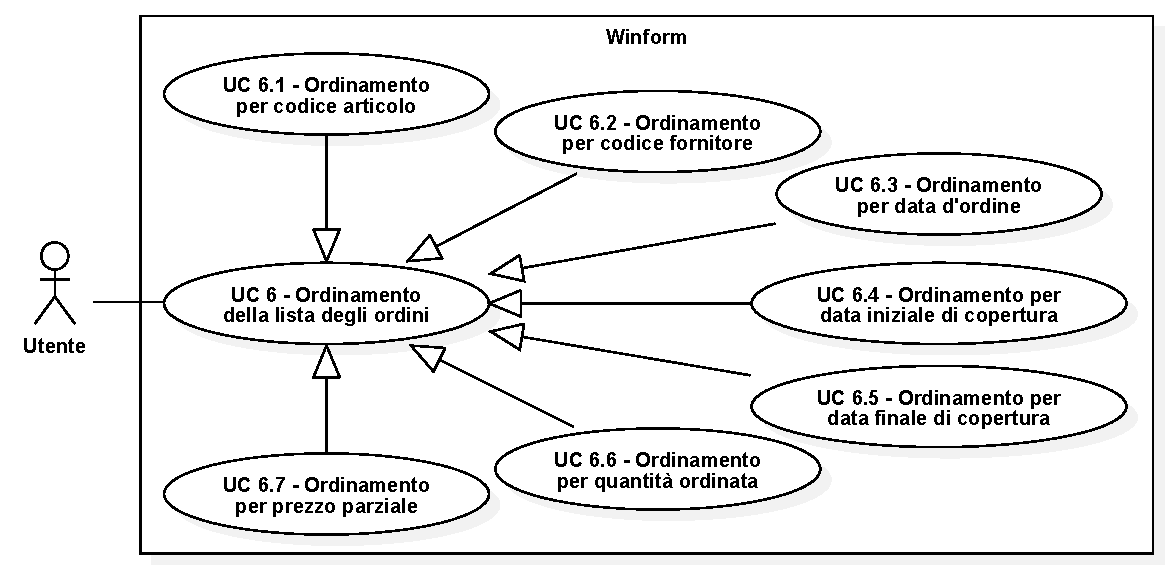
\includegraphics[width=0.95\columnwidth]{usecase/UC 6.pdf} 
    \caption{UC 6 - Ordinamento della lista degli ordini}
\end{figure}
\begin{itemize}

	\item \textbf{Attori primari: }
		\begin{itemize}
			\item Utente.
		\end{itemize}

	\item \textbf{Precondizione: }\\[0.3cm]
		L'utente visualizza correttamente la lista degli ordini.

	\item \textbf{Scenario principale: }
		\begin{enumerate}
			\item L'utente sceglie l'ordinamento da applicare alla lista.
		\end{enumerate}
		

	\item \textbf{Postcondizione: }\\[0.3cm]
		L'utente visualizza correttamente tutti gli elementi ordinati secondo la sua scelta.
    
    \item \textbf{Generalizzazioni: }
        \begin{itemize}
            \item Ordinamento per codice articolo (\hyperref[uc:ordinamento-codice-articolo]{UC 6.1});
            \item Ordinamento per codice fornitore (\hyperref[uc:ordinamento-codice-fornitore]{UC 6.2});
            \item Ordinamento per data d'ordine (\hyperref[uc:ordinamento-data-ordine]{UC 6.3});
            \item Ordinamento per data previsione inizio copertura (\hyperref[uc:ordinamento-data-iniziale-copertura]{UC 6.4});
            \item Ordinamento per data previsione fine copertura (\hyperref[uc:ordinamento-data-finale-copertura]{UC 6.5});
            \item Ordinamento per quantità ordinata (\hyperref[uc:ordinamento-quantita-ordinata]{UC 6.6});
            \item Ordinamento per prezzo parziale (\hyperref[uc:ordinamento-prezzo-parziale-ord]{UC 6.7}).
        \end{itemize}
\end{itemize}

\vspace{0.4cm}

\noindent \textbf{\large UC 6.1 - Ordinamento per codice articolo }
\label{uc:ordinamento-codice-articolo}
\begin{itemize}

	\item \textbf{Attori primari: }
		\begin{itemize}
			\item Utente.
		\end{itemize}

	\item \textbf{Precondizione: }\\[0.3cm]
		L'utente visualizza correttamente la lista degli ordini.
\item \textbf{Scenario principale: }
		\begin{enumerate}
			\item L'utente ordina la lista per codice articolo.
		\end{enumerate}
		

	\item \textbf{Postcondizione: }\\[0.3cm]
		L'utente visualizza correttamente tutti gli elementi ordinati rispetto al codice articolo.

\end{itemize}

\vspace{0.4cm}

\noindent \textbf{\large UC 6.2 - Ordinamento per codice fornitore }
\label{uc:ordinamento-codice-fornitore}
\begin{itemize}

	\item \textbf{Attori primari: }
		\begin{itemize}
			\item Utente.
		\end{itemize}

	\item \textbf{Precondizione: }\\[0.3cm]
		L'utente visualizza correttamente la lista degli ordini.

	\item \textbf{Scenario principale: }
		\begin{enumerate}
			\item L'utente ordina la lista per codice fornitore.
		\end{enumerate}
		

	\item \textbf{Postcondizione: }\\[0.3cm]
		L'utente visualizza correttamente tutti gli elementi ordinati rispetto al codice fornitore.

\end{itemize}

\vspace{0.4cm}

\noindent \textbf{\large UC 6.3 - Ordinamento per data d'ordine }
\label{uc:ordinamento-data-ordine}
\begin{itemize}

	\item \textbf{Attori primari: }
		\begin{itemize}
			\item Utente.
		\end{itemize}

	\item \textbf{Precondizione: }\\[0.3cm]
		L'utente visualizza correttamente la lista degli ordini.

	\item \textbf{Scenario principale: }
		\begin{enumerate}
			\item L'utente ordina la lista per data d'ordine.
		\end{enumerate}
		

	\item \textbf{Postcondizione: }\\[0.3cm]
		L'utente visualizza correttamente tutti gli elementi ordinati rispetto alla data d'ordine.

\end{itemize}

\vspace{0.4cm}

\noindent \textbf{\large UC 6.4 - Ordinamento per data iniziale di copertura }
\label{uc:ordinamento-data-iniziale-copertura}
\begin{itemize}

	\item \textbf{Attori primari: }
		\begin{itemize}
			\item Utente.
		\end{itemize}

	\item \textbf{Precondizione: }\\[0.3cm]
		L'utente visualizza correttamente la lista degli ordini.

	\item \textbf{Scenario principale: }
		\begin{enumerate}
			\item L'utente filtra uno o più ordini per data iniziale di copertura.
		\end{enumerate}
		

	\item \textbf{Postcondizione: }\\[0.3cm]
		L'utente visualizza correttamente tutti gli elementi ordinati rispetto alla data iniziale di copertura.

\end{itemize}

\vspace{0.4cm}

\noindent \textbf{\large UC 6.5 - Ordinamento per data finale di copertura}
\label{uc:ordinamento-data-finale-copertura}
\begin{itemize}

	\item \textbf{Attori primari: }
		\begin{itemize}
			\item Utente.
		\end{itemize}

	\item \textbf{Precondizione: }\\[0.3cm]
		L'utente visualizza correttamente la lista degli ordini.

	\item \textbf{Scenario principale: }
		\begin{enumerate}
			\item L'utente filtra uno o più ordini per data finale di copertura.
		\end{enumerate}
		

	\item \textbf{Postcondizione: }\\[0.3cm]
		L'utente visualizza correttamente tutti gli elementi ordinati rispetto alla data finale di copertura.

\end{itemize}

\vspace{0.4cm}

\noindent \textbf{\large UC 6.6 - Ordinamento per quantità ordinata}
\label{uc:ordinamento-quantita-ordinata}
\begin{itemize}

	\item \textbf{Attori primari: }
		\begin{itemize}
			\item Utente.
		\end{itemize}

	\item \textbf{Precondizione: }\\[0.3cm]
		L'utente visualizza correttamente la lista degli ordini.

	\item \textbf{Scenario principale: }
		\begin{enumerate}
			\item L'utente filtra uno o più ordini per quantità ordinata.
		\end{enumerate}
		

	\item \textbf{Postcondizione: }\\[0.3cm]
		L'utente visualizza correttamente tutti gli elementi ordinati rispetto alla quantità ordinata.

\end{itemize}

\vspace{0.4cm}

\noindent \textbf{\large UC 6.7 - Ordinamento per prezzo parziale}
\label{uc:ordinamento-prezzo-parziale-ord}
\begin{itemize}

	\item \textbf{Attori primari: }
		\begin{itemize}
			\item Utente.
		\end{itemize}

	\item \textbf{Precondizione: }\\[0.3cm]
		L'utente visualizza correttamente la lista degli ordini.

	\item \textbf{Scenario principale: }
		\begin{enumerate}
			\item L'utente ordina gli elementi rispetto al prezzo parziale.
		\end{enumerate}
		

	\item \textbf{Postcondizione: }\\[0.3cm]
		L'utente visualizza correttamente tutti gli elementi ordinati rispetto al prezzo parziale.

\end{itemize}

\vspace{0.4cm}

\section{Tracciamento dei requisiti}

\noindent Da un'attenta analisi dei requisiti e degli use case effettuata sul progetto è stata stilata la tabella che traccia i requisiti in rapporto agli use case.\\
Sono stati individuati diversi tipi di requisiti e si è dunque utilizzato un codice identificativo univoco per distinguerli.\\
Il codice dei requisiti è così strutturato:
\begin{center}
    \textbf{R<NumeroRequisito>-<Tipo>-<Classificazione>}
\end{center}
In particolare il tipo può assumere 4 valori, quali:
\begin{itemize}
    \item \textbf{F} = funzionale
    \item \textbf{Q} = qualitativo
    \item \textbf{P} = performance
    \item \textbf{V} = vincolo
\end{itemize}
Per quanto riguarda la classificazione, invece, si hanno 3 valori possibili:
\begin{itemize}
    \item \textbf{O} = obbligatorio
    \item \textbf{D} = desiderabile
    \item \textbf{F} = facoltativo
\end{itemize}
Nelle tabelle \ref{tab:requisiti-funzionali}, \ref{tab:requisiti-qualitativi}, \ref{tab:requisiti-di-performance} \ref{tab:requisiti-di-vincolo} suddivise per tipo sono riassunti i requisiti e il loro tracciamento con gli use case delineati in fase di analisi.

%comando arraystretch
\renewcommand{\arraystretch}{1.6}

% tab funzionali

\begin{center}
\rowcolors{2}{lightest-grayest}{white}
\begin{longtable}{|p{2cm}|p{9cm}|p{2cm}|}
\caption{Tabella del tracciamento dei requisiti funzionali}
\label{tab:requisiti-funzionali}
\\ \hline
\centering \textbf{Requisito} & \centering \textbf{Descrizione} & \centering \textbf{Use Case} \arraybackslash \\
\hline 
\req{R1-F-O}{L'utente deve poter inserire i dati necessari per l'ottimizzazione}{\hyperref[uc:inserimento-dati]{UC1}}
\req{R2-F-O}{L'utente deve poter inserire la data di inizio previsione}{\hyperref[uc:inserimento-data-inizio-prev]{UC1.1}}
\req{R3-F-O}{L'utente deve poter inserire la data di fine previsione}{\hyperref[uc:inserimento-data-fine-prev]{UC1.2}}
\req{R4-F-O}{L'utente deve poter essere avvisato dell'errore di inserimento della data di inizio previsione}{\hyperref[uc:err-inserimento-data-inizio-prev]{UC1.3}}
\req{R5-F-O}{L'utente deve poter essere avvisato dell'errore di inserimento della data di fine previsione}{\hyperref[uc:err-inserimento-data-fine-prev]{UC1.4}}
\req{R6-F-O}{L'utente deve poter iniziare l'analisi di ottimizzazione}{\hyperref[uc:inizio-analisi-ottimizzazione]{UC2}}
\req{R7-F-O}{L'utente deve poter visualizzare i risultati}{\hyperref[uc:visualizzazione-risultati]{UC3}}
\req{R8-F-O}{L'utente deve poter visualizzare il totale non ottimizzato}{\hyperref[uc:visualizzazione-totale-non-ottimizzato]{UC3.1}}
\req{R9-F-O}{L'utente deve poter visualizzare il totale ottimizzato}{\hyperref[uc:visualizzazione-totale-ottimizzato]{UC3.2}}
\req{R10-F-O}{L'utente deve poter visualizzare lo scostamento tra i totali}{\hyperref[uc:visualizzazione-scostamento-percentuale-totali]{UC3.3}}
\req{R11-F-O}{L'utente deve poter visualizzare la lista degli ordini in maniera decrescente rispetto al codice articolo}{\hyperref[uc:visualizzazione-lista-ordini]{UC4}}
\req{R12-F-O}{L'utente deve poter visualizzare un singolo ordine della lista}{\hyperref[uc:visualizzazione-singolo-ordine]{UC4.1}}
\req{R13-F-O}{L'utente deve poter visualizzare il codice articolo di un ordine}{\hyperref[uc:visualizzazione-codice-articolo]{UC4.1.1}}
\req{R14-F-O}{L'utente deve poter visualizzare il codice fornitore di un ordine}{\hyperref[uc:visualizzazione-codice-fornitore]{UC4.1.2}}
\req{R15-F-O}{L'utente deve poter visualizzare la data d'ordine di un ordine}{\hyperref[uc:visualizzazione-data-ordine]{UC4.1.3}}
\req{R16-F-O}{L'utente deve poter visualizzare la data iniziale di copertura di un ordine}{\hyperref[uc:visualizzazione-data-iniziale-copertura]{UC4.1.4}}
\req{R17-F-O}{L'utente deve poter visualizzare la data finale di copertura di un ordine}{\hyperref[uc:visualizzazione-data-finale-copertura]{UC4.1.5}}
\req{R18-F-O}{L'utente deve poter visualizzare la quantità ordinata di un ordine}{\hyperref[uc:visualizzazione-quantita-ordinata]{UC4.1.6}}
\req{R19-F-O}{L'utente deve poter visualizzare il prezzo parziale di un ordine}{\hyperref[uc:visualizzazione-prezzo-parziale-ord]{UC4.1.7}}
\req{R20-F-O}{L'utente deve poter filtrare la lista}{\hyperref[uc:filtraggio-dati]{UC5}}
\req{R21-F-O}{L'utente deve poter filtrare la lista tramite una ricerca generica}{\hyperref[uc:filtraggio-ricerca-generica]{UC5.1}}
\req{R22-F-O}{L'utente deve poter filtrare la lista per codice articolo}{\hyperref[uc:filtraggio-codice-articolo]{UC5.2}}
\req{R23-F-O}{L'utente deve poter filtrare la lista per codice fornitore}{\hyperref[uc:filtraggio-codice-fornitore]{UC5.3}}
\req{R24-F-O}{L'utente deve poter filtrare la lista per data d'ordine}{\hyperref[uc:filtraggio-data-ordine]{UC5.4}}
\req{R25-F-O}{L'utente deve poter filtrare la lista per data iniziale di copertura}{\hyperref[uc:filtraggio-data-iniziale-copertura]{UC5.5}}
\req{R26-F-O}{L'utente deve poter filtrare la lista per data finale di copertura}{\hyperref[uc:filtraggio-data-finale-copertura]{UC5.6}}
\req{R27-F-O}{L'utente deve poter filtrare la lista per quantità ordinata}{\hyperref[uc:filtraggio-quantita-ordinata]{UC5.7}}
\req{R28-F-O}{L'utente deve poter filtrare la lista per prezzo parziale}{\hyperref[uc:filtraggio-prezzo-parziale-ord]{UC5.8}}
\req{R29-F-O}{L'utente deve poter ordinare la lista degli ordini}{\hyperref[uc:ordinamento-elementi-lista]{UC6}}
\req{R30-F-O}{L'utente deve poter ordinare la lista rispetto al codice articolo}{\hyperref[uc:ordinamento-codice-articolo]{UC6.1}}
\req{R31-F-O}{L'utente deve poter ordinare la lista rispetto al codice fornitore}{\hyperref[uc:ordinamento-codice-fornitore]{UC6.2}}
\req{R32-F-O}{L'utente deve poter ordinare la lista rispetto alla data d'ordine}{\hyperref[uc:ordinamento-data-ordine]{UC6.3}}
\req{R33-F-O}{L'utente deve poter ordinare la lista rispetto alla data iniziale di copertura}{\hyperref[uc:ordinamento-data-iniziale-copertura]{UC6.4}}
\req{R34-F-O}{L'utente deve poter ordinare la lista rispetto alla data finale di copertura}{\hyperref[uc:ordinamento-data-finale-copertura]{UC6.5}}
\req{R35-F-O}{L'utente deve poter ordinare la lista rispetto alla quantità ordinata}{\hyperref[uc:ordinamento-quantita-ordinata]{UC6.6}}
\req{R36-F-O}{L'utente deve poter ordinare la lista rispetto al prezzo parziale}{\hyperref[uc:ordinamento-prezzo-parziale-ord]{UC6.7}}
\end{longtable}
\end{center}%

%tab qualità
\begin{center}
\rowcolors{2}{lightest-grayest}{white}
\begin{longtable}{|p{2cm}|p{9cm}|p{2cm}|}
\caption{Tabella del tracciamento dei requisiti qualitativi}
\label{tab:requisiti-qualitativi}
\\ \hline
\centering \textbf{Requisito} & \centering \textbf{Descrizione} & \centering \textbf{Use Case} \arraybackslash \\
\hline 
\req{R37-Q-O}{Deve essere redatto un documento che descrive l'architettura del modulo}{-}
\req{R38-Q-O}{Deve essere redatto un documento che spieghi le scelte implementative effettuate}{-}
\req{R39-Q-O}{Il codice deve essere documentato tramite commenti}{-}
\req{R40-Q-D}{L'algoritmo finale scelto deve generare dei log di chiamata per manutenzioni future}{-}
\req{R41-Q-D}{L'algoritmo di ottimizzazione deve essere estensibile}{-}
\req{R42-Q-O}{I test devono coprire il 60\% del codice}{-}
\req{R43-Q-D}{L'algoritmo utilizza differenti tecniche di ottimizzazione}{-}
\req{R44-Q-F}{L'algoritmo utilizza il multithreading per cercare più soluzioni ammissibili}{-}
\end{longtable}
\end{center}%

%tab performance
\begin{center}
\rowcolors{2}{lightest-grayest}{white}
\begin{longtable}{|p{2cm}|p{9cm}|p{2cm}|}
\caption{Tabella del tracciamento dei requisiti di performance}
\label{tab:requisiti-di-performance}
\\ \hline
\centering \textbf{Requisito} & \centering \textbf{Descrizione} & \centering \textbf{Use Case} \arraybackslash \\
\hline 
\req{R45-P-O}{L'algoritmo di ottimizzazione deve restituire un risultato entro 10 minuti dal tempo di lancio dello stesso}{-}
\end{longtable}
\end{center}%

%tab vincolo
\begin{center}
\rowcolors{2}{lightest-grayest}{white}
\begin{longtable}{|p{2cm}|p{9cm}|p{2cm}|}
\caption{Tabella del tracciamento dei requisiti di vincolo}
\label{tab:requisiti-di-vincolo}
\\ \hline
\centering \textbf{Requisito} & \centering \textbf{Descrizione} & \centering \textbf{Use Case} \arraybackslash \\
\hline  
\req{R46-V-O}{La \textit{form} deve essere eseguita sull'ambiente di esecuzione \textit{.NET Framework}}{-}
\req{R47-V-O}{La \textit{form} e l'algoritmo devono essere codificate in $C\#$}{-}
\req{R48-V-O}{La versione utilizzata di $C\#$ deve essere $7.3$}{-}
\req{R49-V-O}{La versione utilizzata di \textit{.NET Framework} deve essere $4.8$}{-}
\req{R50-V-O}{L'algoritmo finale deve fonire una soluzione ammissibile}{-}
\end{longtable}
\end{center}%             % Concept Preview
% !TEX encoding = UTF-8
% !TEX TS-program = pdflatex
% !TEX root = ../tesi.tex

\newgeometry{a4paper, left=30mm, right=30mm, top=5mm, bottom=30mm}
%**************************************************************
\chapter{Progettazione e codifica}
\label{cap:progettazione-codifica}
%**************************************************************

\noindent \intro{In questo capitolo vengono esposte le attività di progettazione e codifica del modulo di ottimizzazione}\\

%**************************************************************
\section{Architettura}
\label{sec:progettazione}
\noindent Prima di descrivere più in particolare l'algoritmo, è necessario
fornire un’idea dell’architettura sulla quale si basa l'intero progetto.
Di seguito è presentato uno schema ad alto livello di come sono strutturate le varie
componenti che formano il sistema.

\begin{figure}[!h] 
    \centering 
    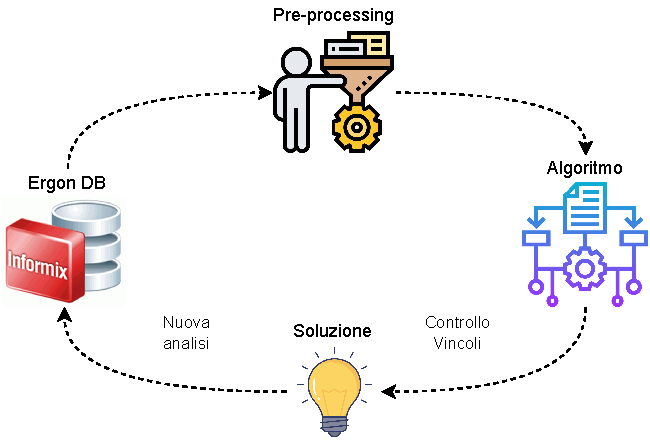
\includegraphics[width=0.95\columnwidth]{architettura/architettura.pdf} 
    \caption{Architettura generale}
    \label{architettura-generale}
\end{figure}

\noindent Come si può notare in figura \ref{architettura-generale},
il flusso del sistema è circolare.
Si parte dal database, dal quale vengono estratti i dati di interesse dalle varie
tabelle. Successivamente viene fatto il pre-processing dei dati,
in modo tale da poter poi eseguire l'ottimizzazione solo su
ciò che è di interesse dell'analisi.
Di seguito viene effettuato il controllo dei vincoli di minimo al termine
dell'algoritmo così da generare
una soluzione ammissibile. Se si vuole effettuare una nuova
analisi è necessario estrarre nuovamente i dati dal
database ed eseguire nuovamente il ciclo. Questo è necessario
in quanto i dati all'interno del database possono variare
(esempio: prezzi, date di spedizione...).

\newpage

\newgeometry{a4paper, left=30mm, right=30mm, top=31mm, bottom=30mm}

\section{Funzionamento generale}
In questa sezione viene descritta una classica interazione dell'utente con il programma.
Nella figura \ref{diagramma-attivita-winform} si riassume il flusso delle interazioni.

\begin{figure}[!h] 
    \centering 
    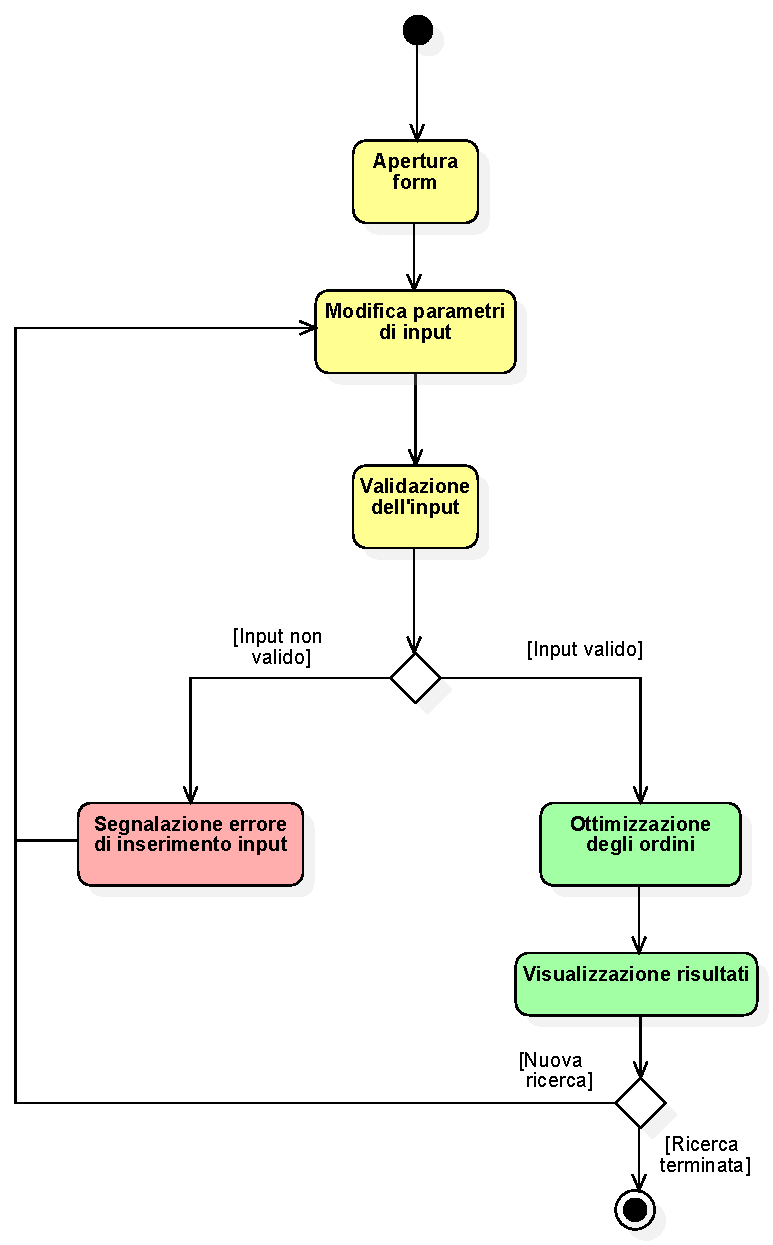
\includegraphics[scale = 0.75]{diagrammi attivita/Diagramma di attivita winform.pdf} 
    \caption{Diagramma di attività della WinForm}
    \label{diagramma-attivita-winform}
\end{figure}

\noindent L'utente, all'apertura della WinForm, modifica i parametri di input che sono:
\begin{itemize}
    \item data di previsione iniziale
    \item data di previsione finale
    \item metodo di risoluzione dei vincoli
\end{itemize}
\noindent Dopo aver scelto gli input, questi vengono validati in modo tale da bloccare anzitempo
l'esecuzione in caso di errori.
Se la validazione va a buon fine allora l'algoritmo calcola la soluzione e vengono visualizzati i risultati.
A questo punto la ricerca può terminare oppure può continuare con la possibilità di variare i parametri di input.

%**************************************************************
\section{Tabu Search}
\label{sec:tabu-search}
\noindent Nella sezione § \ref{conclusione-studio-fattibilita}
riguardante lo studio di fattibilità è emerso come la tabu search
sia il giusto compromesso in termini di efficacia, efficienza
e complessità a livello implementativo.\\
In figura \ref{diagramma-attivita-tabu-search}
viene rappresentato il funzionamento dell'algoritmo ad alto livello.
\vspace*{\fill}
\begin{figure}[!h] 
    \centering 
    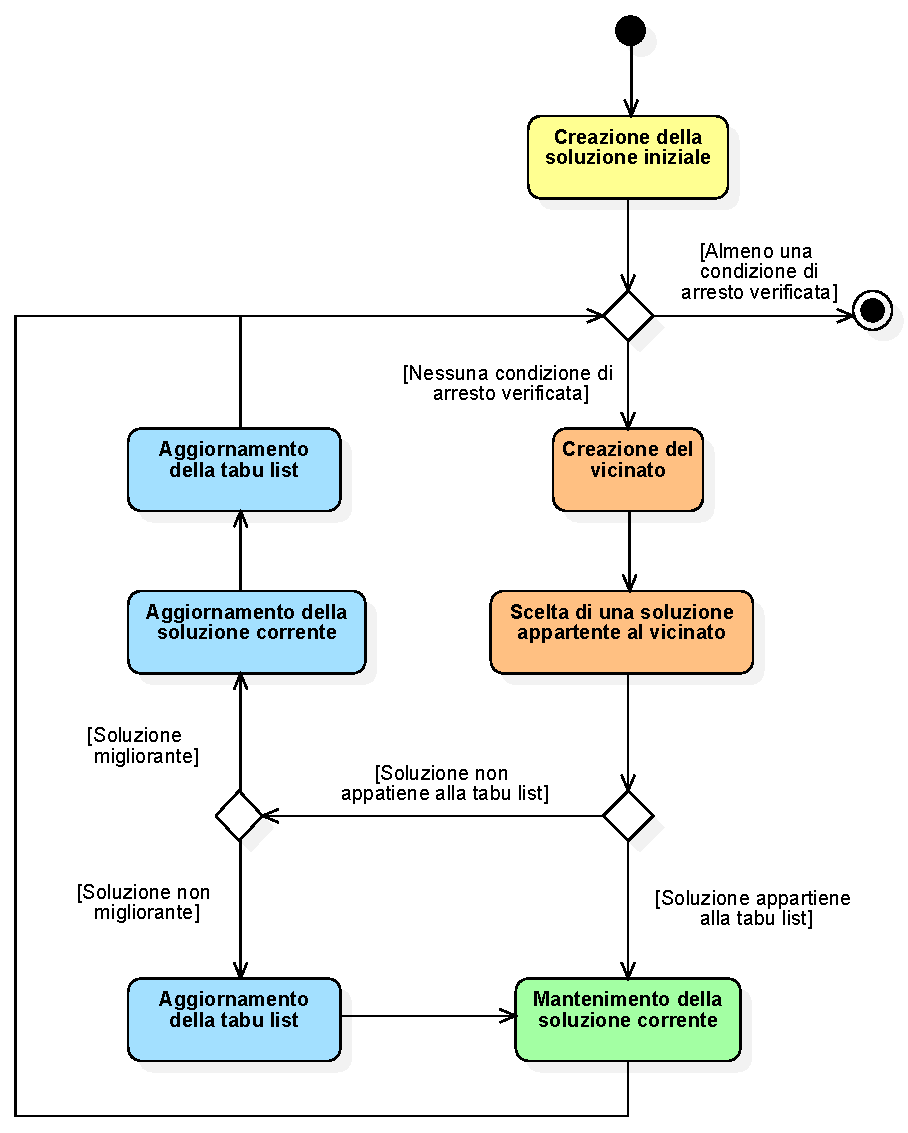
\includegraphics[width=0.8\columnwidth]{diagrammi attivita/diagramma attivita tabusearch.pdf} 
    \caption{Diagramma di attività della tabu search}
    \label{diagramma-attivita-tabu-search}
\end{figure}
\noindent \paragraph{}\hfill\\
Come si può notare, prima viene effettuato un controllo per vedere se la mossa
appartiene o meno alla tabu list e poi viene verificato se la soluzione è migliorante.
Se i controlli venissero invertiti, si rischierebbe, calcolando
la funzione di valutazione e confrontandola con quella della soluzione corrente,
di simulare inutilmente una mossa che potenzialmente potrebbe appartenere alla tabu list.
\vspace*{\fill}

\newpage

%**************************************************************
\subsection{Rappresentazione della soluzione}
\label{sec:rappresentazione-della-soluzione}
\noindent Definire una buona rappresentazione della soluzione è fondamentale
poichè è legata alla creazione del vicinato.\\
In primis è stata creata una classe che rappresentasse
il singolo ordine (dataSourceItem) e, dato che gli ordini solitamente sono molteplici,
si è deciso di mettere ognuno di essi all'interno di una lista.
Questo approccio è sufficiente per un algoritmo greedy, ma non per la tabu search.\\
Infatti è necessario associare alla soluzione anche una funzione di valutazione, in modo tale
da poter operare il confronto tra la soluzione corrente e quella migliore.\\
In figura \ref{rappresentazione-soluzione} viene illustrata la forma della soluzione della tabu search.
\begin{figure}[!h] 
    \centering 
    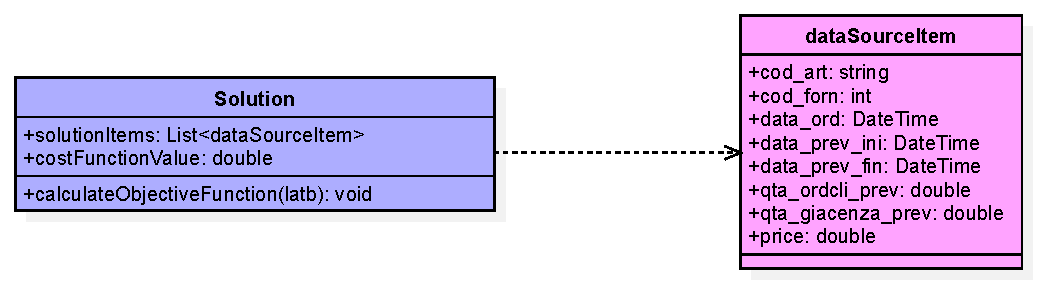
\includegraphics[width=0.8\columnwidth]{soluzione/soluzione rappresentazione.pdf} 
    \caption{Rappresentazione della soluzione per la tabu search}
    \label{rappresentazione-soluzione}
\end{figure}

%**************************************************************
\subsection{Soluzione iniziale}
\label{sec:soluzione-iniziale}
\noindent Nella figura \ref{diagramma-attivita-tabu-search} il primo step è la creazione di una soluzione iniziale che
però la tabu search, a contrario di altri algoritmi, non è in grado di generare da sola. Per ovviare a questo inconveniente
si può generare una soluzione abbastanza buona tramite un algoritmo greedy.\\
Di seguito viene presentato lo pseudocodice.
\vspace*{\fill}
\begin{algorithm}
    \captionsetup{labelformat=empty}
    \caption{Pseudocodice soluzione iniziale - Algoritmo Greedy}
    \vspace{0.1cm}
    \hspace*{\algorithmicindent} \textbf{Input:} {$lista\_articoli$}, {$lista\_spedizioni$}, {$lista\_prezzi$}\\
    \hspace*{\algorithmicindent} \textbf{Output:} {$lista\_articoli\_opt$}
    \begin{algorithmic}[1]
        \Procedure{My\_Greedy\_Algorithm}{$lista\_articoli$, $lista\_spedizioni$, $lista\_prezzi$}
        \State {$l \gets lista\_vuota$}
        \State {$l_{tmp} \gets lista\_vuota$}
        \State $l_{cod\_art} \gets genera\_lista\_decisione(lista\_articoli)$
        \State $n_{cod\_art} \gets l_{cod\_art}.Length$
        \While {$count < n_{cod\_art}$}
            \State {$cod\_art \gets decisione(l_{cod\_art})$}
            \ForAll {$art \in lista\_articoli$}
                \State {$b \gets controllo\_condizioni(art$, $cod\_art$, $lista\_spedizioni$, $lista\_prezzi)$}
                \If {$b = true$}
                    \State Aggiungi $art$ a $l_{tmp}$
                \EndIf
            \EndFor
            \State {$count \gets count+1$}
        \EndWhile
        \State $l \gets filtra\_articoli\_per\_min(l_{tmp})$
        \State \Return $l$
        \EndProcedure
    \end{algorithmic}
\end{algorithm}
\vspace*{\fill}
\newpage
\noindent Si può notare come la funzione $controllo\_condizioni()$ abbia lo scopo di escludere tutte le casistiche relative a tutti i $cod\_art$ in cui:
\begin{itemize}
    \item la data di spedizione è minore del giorno attuale
    \item la data di arrivo della spedizione è maggiore della data di inizio copertura
    \item dato un fornitore, non esiste un prezzo associato ad alcuna spedizione
    \item dato un fornitore, non esiste alcuna spedizione associata ad un prezzo
\end{itemize}

\noindent La funzione $filtra\_articoli\_per\_min()$, avente come parametro di input $l_{tmp}$ (lista con tutti i record che soddisfano i vincoli),
serve invece a filtrare per prezzo minimo tutti i range di copertura associati ad ogni codice articolo.
In pratica per ogni range di copertura di ogni articolo viene preso il record con il fornitore che offre il fabbisogno al prezzo più vantaggioso.\\

\noindent É possibile avere anche un'inizializzazione della soluzione che non sia stata soggetta ad alcuna ottimizzazione.
In questo caso è stata creata una funzione $initialise\_solution()$ che, dati in input gli stessi parametri dell'algoritmo greedy, fornisce
come soluzione iniziale proprio quella generata dal modulo già esistente. 

%**************************************************************
\subsection{Mosse}
\label{sec:mosse}
\noindent Le mosse create per la Tabu Search sono le seguenti:
\begin{enumerate}
    \item Inserimento di un nuovo ordine d'acquisto
    \item Cambio di fornitore di un ordine d'acquisto
    \item Pre-ordine di un ordine d'acquisto
    \item Post-ordine di un ordine d'acquisto
\end{enumerate}
Come si può notare non è stata creata la mossa inversa dell'inserimento, ovvero la rimozione di un ordine d'acquisto.
Il motivo sta nel fatto che rimuovere un ordine di un articolo di cui si ha bisogno non porta sicuramente a un miglioramento
della funzione di valutazione poichè, essendo l'articolo una necessità, prima o poi verrà aggiunto nuovamente.

%**************************************************************
\subsection{Esplorazione del vicinato}
\label{sec:esplorazione-vicinato}
\noindent Il vicinato è quell'insieme di soluzioni che possono essere raggiunte
tramite l'applicazione di una mossa sulla soluzione corrente (chiamata anche centro del vicinato).\\
Si può notare come la dimensione del vicinato in questo problema sia dell'ordine di $O(n!)$ e sia dettata dal fatto che
per ogni range di copertura di ogni articolo sia necessario scegliere la miglior
combinazione tra data d'ordine e fornitore.\\
Data la sua alta complessità non è dunque possibile visitare l'intero vicinato,
motivo per il quale si è deciso di procedere randomizzando le scelte.
In particolare ogni mossa viene selezionata in maniera casuale cosicché tutte le scelte
abbiano la stessa probabilità di essere selezionate.\\
Per lo stesso motivo è stato applicato lo stesso principio anche per la scelta dell'articolo su cui applicare
la mossa.

%**************************************************************
\subsection{Tabu List}
\label{sec:tabu-list}
\noindent La tabu list è una lista che memorizza le k mosse precedenti, dove k è uguale
alla lunghezza della lista che viene definita alla creazione dell'oggetto \textit{TabuSearch}.\\
Permette di evitare dunque cicli infiniti in corrispondenza
di minimi locali. Questo accade perché tramite le funzione $generate\_move\_string()$ ogni mossa
viene prima codificata, poi viene effettuata una ricerca nella tabu list, impedendo potenzialmente all’algoritmo di riprovarla,
e infine viene aggiunta nella lista sia nel caso in cui venga effettuata che nel caso in cui non venga effettuata perchè non migliorante.\\
Per semplificare la codifica si salva solamente la stringa generata dalla funzione che rappresenta la mossa e non l’intera
soluzione come previsto dalla teoria.
Si è deciso inoltre di memorizzare, oltre alla mossa eseguita, anche la sua inversa
(per esempio l'inversa del pre-ordine è il post-ordine). Così facendo si
evitano le inversioni immediate che risulterebbero poco sensate e rallenterebbero la ricerca.

%**************************************************************
\subsection{Funzione di valutazione}
\label{sec:funzione-valutazione}
\noindent I parametri da considerare per valutare la bontà di una soluzione, vista dal lato utente,
sono i seguenti:
\begin{itemize}
    \item il numero di articoli ordinati rispetto a quelli totali
    \item il prezzo totale di tutti gli ordini effettuati
\end{itemize}
Chiaramente la funzione di valutazione deve migliorare
se aumenta il numero di articoli ordinati
oppure il prezzo totale diminuisce a parità di articoli ordinati.
Al contrario si ha un peggioramento nel caso in cui a parità di articoli ordinati
corrisponde un prezzo totale maggiore. Non si potrà mai
avere invece un peggioramento della funzione di valutazione causato dalla diminuzione del numero di articoli
ordinati, come spiegato nella sezione §\ref{sec:mosse}.\\
La funzione di valutazione, in questo caso, non può rappresentare perfettamente il
comportamento dell'algoritmo e definisce dunque un'approssimazione del suo andamento.\\
Di seguito vengono riportati i test effettuati per capire empiricamente quale fosse la funzione di valutazione
che approssimasse meglio il comportamento dell'algoritmo.

%tab vincolo
\begin{center}
    \rowcolors{2}{lightest-grayest}{white}
    \begin{longtable}{|m{1.2cm}|m{1.6cm}|m{1cm}|m{1.7cm}|}
    \caption{Tabella dei risultati della funzione }
    \label{tab:risultati-funzione-lineare}
    \\ \hline
    \rowcolor{lighter-grayer}
    \centering \textbf{PT} & \multicolumn{2}{c}{\centering \textbf{Rapporto $\frac{OE}{OT}$}} & \centering \textbf{FV} \arraybackslash \\
    \hline
    \fval{100.000}{10}{0,0076}{11,3368318}
    \fval{200.000}{20}{0,0153}{11,8348101}
    \fval{300.000}{30}{0,0230}{11,8653914}
    \fval{400.000}{40}{0,0307}{12,1234943}
    \fval{500.000}{50}{0,0384}{12,1415785}
    \fval{600.000}{60}{0,0461}{12,1182141}
    \fval{350.000}{21}{0,0161}{12,3582223}
    \fval{350.000}{22}{0,0169}{12,3390647}
    \fval{350.000}{23}{0,0176}{12,3199292}
    \fval{400.000}{23}{0,0176}{12,4487975}
    \fval{400.000}{24}{0,0184}{12,4294842}
    \fval{500.000}{1300}{1,0000}{-0,0000020}
    \fval{450.000}{1300}{1,0000}{-0,0000022}
    \end{longtable}
\end{center}
\begin{center}
    %tab vincolo
    \rowcolors{2}{lightest-grayest}{white}
    \begin{longtable}{|m{1.2cm}|m{1.6cm}|m{1cm}|m{1.7cm}|}
    \caption{Tabella dei risultati della funzione }
    \label{tab:risultati-funzione-lineare}
    \\ \hline
    \rowcolor{lighter-grayer}
    \centering \textbf{PT} & \multicolumn{2}{c}{\centering \textbf{Rapporto $\frac{OE}{OT}$}} & \centering \textbf{FV} \arraybackslash \\
    \hline
    \fval{100.000}{10}{0,0076}{11,3368318}
    \fval{200.000}{20}{0,0153}{11,8348101}
    \fval{300.000}{30}{0,0230}{11,8653914}
    \fval{400.000}{40}{0,0307}{12,1234943}
    \fval{500.000}{50}{0,0384}{12,1415785}
    \fval{600.000}{60}{0,0461}{12,1182141}
    \fval{350.000}{21}{0,0161}{12,3582223}
    \fval{350.000}{22}{0,0169}{12,3390647}
    \fval{350.000}{23}{0,0176}{12,3199292}
    \fval{400.000}{23}{0,0176}{12,4487975}
    \fval{400.000}{24}{0,0184}{12,4294842}
    \fval{500.000}{1300}{1,0000}{-0,0000020}
    \fval{450.000}{1300}{1,0000}{-0,0000022}
    \end{longtable}
\end{center}

%**************************************************************
\subsection{Condizioni di arresto}
\label{sec:condizioni-arresto}
\noindent La Tabu Search si ferma se si verifica almeno una delle seguenti condizioni:
\begin{itemize}
    \item \textbf{Numero massimo di iterazioni:} numero di mosse eseguibili dall'algoritmo, deciso
    dal programmatore, che permette di evitare la possibilità di eventuali cicli infiniti;
    \item \textbf{Numero massimo di iterazioni non migliorative:} numero di mosse non migliorative
    consecutive eseguibili dall'algoritmo, deciso dal programmatore, che permette
    di rilevare in maniera approssimativa un minimo
    locale e terminare la procedura;
    \item \textbf{Tempo massimo di esecuzione:}  durata temporale oltre
    la quale il programma si ferma automaticamente. Questo serve per venire incontro a
    bisogni di rapidità di risposta da parte dell’azienda.
    
\end{itemize}
%**************************************************************
\subsection{Controllo dei vincoli}
\label{sec:controllo-vincoli}

%**************************************************************
\section{Codifica}
\label{sec:codifica}

%**************************************************************
\subsection{Organizzazione dello sviluppo}
\label{sec:organizzazione-sviluppo}

%**************************************************************
\subsection{Log}
\label{sec:log}

%**************************************************************
\subsection{Problematiche riscontrate}
\label{sec:problematiche-riscontrate}

%**************************************************************
\subsection{Estensioni del progetto}
\label{sec:estensioni-progetto}

\newpage

%**************************************************************
\section{Tecnologie e strumenti}
\label{sec:tecnologie-strumenti}

\noindent Di seguito viene esposta una panoramica delle tecnologie e degli strumenti utilizzati.
Sono stati tutti imposti da Ergon Informatica in quanto sono le tecnologie e gli strumenti
da loro impiegati per lo sviluppo software.\\
Per l’azienda le caratteristiche determinanti della scelta di queste tecnologie
sono riconducibili alle soddisfazione delle seguenti necessità e aspettative:
\begin{itemize}
    \item compatibilità con il sistema Ergdis;
    \item facilità di apprendimento;
    \item ampia disponibilità della documentazione;
    \item gradevolezza dell’interfaccia grafica.
\end{itemize}
Di seguito vegono presentate le tecnologie utilizzate.


\subsection*{C\#}
\begin{figure}[!h] 
    \centering 
    
\includegraphics[scale = 0.04]{loghi/CSharpLogo.pdf} 
    \caption{Logo C\#}
 \end{figure}
\noindent C\# è un linguaggio di programmazione multi-paradigma orientato agli oggetti
sviluppato da Microsoft. La sua sintassi e struttura derivano da altri linguaggi nati
precedentemente, come C++, Java e Visual Basic.\\
C\# è progettato per essere compatibile con le classi e l’ambiente di compilazione
del framework .NET. Supporta astrazione, ereditarietà e polimorfismo
fornendo estensibilità e riusabilità del codice.
È stato ufficialmente approvato come standard dalla ECMA.\\
L'azienda, sebbene abbia sviluppato la maggior parte dei moduli
in Visual Basic, sta lentamente traducendo tutto in questo linguaggio.

\subsection*{Visual Studio 2019}
\begin{figure}[!h] 
    \centering 
    
\includegraphics[scale = 0.75]{loghi/VisualStudio2019Logo.pdf} 
    \caption{Logo Visual Studio 2019}
 \end{figure}
\noindent Visual Studio 2019 è un ambiente di sviluppo integrato (IDE) fornito da Microsoft.
Permette lo sviluppo di software per computer, siti web, applicazioni web, servizi web
e applicazioni mobile. È compatibile con tutte le piattaforme di sviluppo
software Microsoft, quali Windows API e Windows Form.\\
Visual Studio 2019 supporta il refactoring del codice e intellisense, uno strumento per
l’autocompletamento del codice. Il debugger integrato funziona sia a
livello di codice sorgente che a livello di codice macchina. È compatibile anche con i sistemi di supporto per il controllo del codice,
come per esempio Subversion e Git.\\
Visual Studio 2019 supporta 36 differenti linguaggi di 
programmazione tra i quali C\#.

\subsection*{DevExpress}
\begin{figure}[!h] 
    \centering 
    
\includegraphics[scale = 0.35]{loghi/DevExpressLogo.png}
    \caption{Logo DevExpress}
\end{figure}
\noindent DevExpress è una compagnia che produce strumenti di sviluppo software per
Visual Studio. In particolare crea estensioni che vengono utilizzate tramite Visual
Studio per velocizzare la scrittura di applicazioni. Gli strumenti da loro forniti sono
molteplici, in particolare hanno sviluppato controlli .NET di interfaccia utente (UI).
Questi ultimi rendono più semplice la creazione di ambienti grafici per applicazioni ed
elegante il risultato.

\subsection*{Informix}
\begin{figure}[!h] 
    \centering 
    
\includegraphics[scale = 0.04]{loghi/InformixLogo.pdf}
    \caption{Logo IBM Informix}
\end{figure}
\noindent IBM Informix è un prodotto di IBM. La base di dati Informix è usata in molte
applicazioni OLTP ad alto tasso di transazione che operano in vari settori tra cui anche quelli della produzione e dei trasporti.\\
L’Informix server supporta il modello relazionale ad oggetti che permette ad IBM di
offrire estensioni che permettono di effettuare interrogazioni per un dominio specifico
e archiviazioni per set di dati in maniera rapida ed efficiente.
É in grado di supportare sia SQL che NoSQL.

\subsection*{Git}
\begin{figure}[!h] 
    \centering 
    
\includegraphics[scale = 0.4]{loghi/GitLogo.pdf}
    \caption{Logo Git}
\end{figure}
\noindent Git è uno strumento per il controllo di versione distribuito del codice sorgente delle repository.\\
Creato inizialmente per gestire le versioni del kernel Linux, al giorno d'oggi è uno dei principali
strumenti di versionamento del codice e di collaborazione tra gli sviluppatori.
             % Product Prototype
% !TEX encoding = UTF-8
% !TEX TS-program = pdflatex
% !TEX root = ../tesi.tex

%**************************************************************
\chapter{Verifica e validazione}
\label{cap:verifica-validazione}

%**************************************************************
\section{Verifica}

%**************************************************************
\subsection{Documentazione}

%**************************************************************
\subsection{Testing del modulo}

%**************************************************************
\section{Validazione}

%**************************************************************
\subsection{Documentazione}

%**************************************************************
\subsection{Codice}

%**************************************************************             % Product Design Freeze e SOP
% !TEX encoding = UTF-8
% !TEX TS-program = pdflatex
% !TEX root = ../tesi.tex

\newgeometry{a4paper, left=30mm, right=30mm, top=5mm, bottom=30mm}
%**************************************************************
\chapter{Conclusioni}
\label{cap:conclusioni}
%**************************************************************
\noindent \intro{In questo ultimo capitolo viene effettuata una analisi retrospettiva sullo \textit{stage}
focalizzandosi sul raggiungimento degli obiettivi, sulle conoscenze acquisite e sulla valutazione personale del percorso.}
%**************************************************************
\section{Prodotto finale}
\noindent Come descritto nei capitoli precedenti, il prodotto finale consiste in una \textit{\gls{windowsformg}} che
ottimizza l'insieme degli ordini che vengono effettuati per soddisfare i
fabbisogni di un dato periodo.\\

\noindent Dopo aver inserito tutti gli \textit{input} necessari,
viene determinata una soluzione iniziale tramite un algoritmo \textit{greedy} e poi, attraverso la
\textit{Tabu search}, si crea una nuova soluzione che viene visualizzata in una lista
filtrabile contenente tutte le informazioni di ogni ordine.
%**************************************************************
\section{Raggiungimento degli obiettivi}
\noindent Come descritto nella sezione §\ref{sec:validazione-requisiti}, il prodotto
soddisfa la maggior parte delle necessità descritte nell'analisi dei requisiti.
In particolare sono stati realizzati tutti i requisiti funzionali, la maggior parte
di quelli qualitativi, tutti quelli di performance e di vincolo.\\
Nella tabella \ref{tab:requisiti-riepilogo-validazione} viene fornita una chiara visuale
del soddisfacimento dei requisiti.
\begin{center}
    \rowcolors{2}{lightest-grayest}{white}
    \begin{longtable}{|p{2.5cm}|p{2.5cm}|p{2.5cm}|p{2.5cm}|}
    \caption{Riepilogo della validazione dei requisiti}
    \label{tab:requisiti-riepilogo-validazione}
    \\ \hline
    \rowcolor{lighter-grayer}
    \centering \textbf{Tipo} & \centering \textbf{Obbligatori} & \centering \textbf{Desiderabili} & \centering \textbf{Facoltativi}\arraybackslash \\
    \hline
    \reqsum{Soddisfatti}{45}{2}{0}
    \reqsum{Non Soddisfatti}{0}{2}{1}
    \end{longtable}
\end{center}%
%**************************************************************
\section{Conoscenze acquisite}
\noindent Per la realizzazione di questo progetto sono state fondamentali
molte nozioni apprese durante il corso di studi, dai linguaggi ai paradigmi.\\
Lo \textit{stage} ha permesso però anche di incrementare notevolmente il mio bagaglio
sia tecnico che personale.
Vengono ora elencate le principali conoscenze acquisite.
\paragraph{\textit{Informix}, \textit{C\#} e \textit{MSTest}}\hfill\\\\
\noindent Per lo sviluppo del progetto mi sono servito principalmente di queste tecnologie:
\begin{itemize}
    \item \textit{Informix} per \textit{database}
    \item \textit{C\#} come linguaggio di programmazione
    \item \textit{MSTest} come \textit{framework} di \textit{test}
\end{itemize}
\newgeometry{a4paper, left=30mm, right=30mm, top=31mm, bottom=30mm}
\noindent Non avendole mai affrontate né all’università né in privato ho dovuto
cominciare praticamente da zero, ma poichè struttura, regole e utilizzo sono simili
a tecnologie conosciute, come ad esempio \textit{MySQL} per \textit{Informix}, \textit{C++} e \textit{Java} per \textit{C\#},
e \textit{JUnit} per \textit{MSTest}, l’apprendimento è stato molto semplificato.
Ciò mi ha permesso di acquisire le conoscenze necessarie in tempi rapidissimi
e grazie anche all'utilizzo di un approccio conosciuto come \textit{learning
by doing}.
\paragraph{Analisi e modellazione del problema}\hfill\\\\
Analizzare e modellare un problema è una delle competenze che si devono apprendere
in un corso di laurea in informatica. Tuttavia i problemi con cui si ha a che fare
nel mondo accademico sono molto spesso \textit{standard} e risolvibili tramite tecniche
ben conosciute.\\
Questo progetto mi ha posto davanti per la prima volta un problema
non banale da risolvere da solo. Infatti uno studio preliminare forse poco accurato
mi ha portato a effettuare per buona parte dello \textit{stage} molte domande al \textit{tutor}.
É chiaro dunque come sia fondamentale capire il problema che si ha di fronte nella
sua completa interezza prima di iniziare la progettazione e lo sviluppo.

\paragraph{Gestione delle risorse}\hfill\\\\
Il mondo universitario pone lo studente a organizzare le sue risorse temporali disponibili
per preparare al meglio gli esami. Tutto ciò non ha nulla a che vedere con la
gestione delle risorse in ambito aziendale. L'organizzazione diventa fondamentale
e la schedulazione degli eventi e degli obiettivi diventa imprescindibile.
Lo svolgimento dello \textit{stage} mi ha permesso dunque di crescere molto su questo aspetto
che avevo già rafforzato nel corso di \textit{Ingegneria del software}.

%**************************************************************
\section{Valutazione complessiva}
\noindent Lo \textit{stage} presso \textit{Ergon Informatica} lo valuto in maniera molto positiva.\\
I due mesi trascorsi in azienda sono risultati molto leggeri e piacevoli soprattutto grazie
ad un ambiente di lavoro molto motivante e, a tratti, anche divertente.\\

\noindent Grazie ad un ottimo rapporto con il \textit{\textit{tutor}} aziendale, non ho mai dovuto
affrontare difficoltà bloccanti in autonomia. Gianluca, anche durante il suo periodo di vacanza, è sempre stato disponibile
ad ascoltare dubbi e perplessità per fornirmi indicazioni utili che mi guidassero
verso la via corretta e mi permettessero di continuare il lavoro.\\
Un altro aspetto che ho molto apprezzato è stato l'interesse di alcuni colleghi
verso il progetto che stavo realizzando, il che mi faceva sentire parte integrante
dell'azienda.\\

\noindent Per quanto concerne la parte di realizzazione del progetto, tutto è proseguito secondo quanto programmato.\\
Personalmente ho trovato più difficile la parte di inquadramento del problema e di scelta della funzione di valutazione.
Quest'ultima è stata particolarmente complessa perchè non esisteva una qualche procedura
che descrivesse come arrivare a definire la funzione di valutazione, ma bisognava
effettuare delle prove empiriche e aggiustare la funzione tentativo dopo tentativo.
Ho avuto modo di affrontare tematiche nuove legate alla risoluzione di problemi
relativi al mondo reale e questo mi ha permesso di rimanere costantemente motivato.\\

\noindent Concludendo, questo progetto di \textit{stage} è stato per me
molto soddisfacente per modalità di svolgimento, per il prodotto finale, per le conoscenze acquisite e per le persone conosciute.             % Conclusioni
%\appendix
%% !TEX encoding = UTF-8
% !TEX TS-program = pdflatex
% !TEX root = ../tesi.tex

%**************************************************************
\chapter{Appendice A}
%**************************************************************

\epigraph{Citazione}{Autore della citazione}



             % Appendice A

%**************************************************************
% Materiale finale
%**************************************************************
\backmatter
\printglossary[type=main, title=Glossario, toctitle=Glossario]
% !TEX encoding = UTF-8
% !TEX TS-program = pdflatex
% !TEX root = ../tesi.tex

%**************************************************************
% Bibliografia
%**************************************************************

\cleardoublepage
\chapter{Bibliografia}

% Stampa i riferimenti bibliografici
\printbibliography[heading=subbibliography,title={Riferimenti bibliografici},type=book]

% Stampa i siti web consultati
\printbibliography[heading=subbibliography,title={Siti web consultati},type=online]


\end{document}
